% !TEX program = xelatex
\documentclass[12pt, a4paper, oneside]{book}
% !TEX root = ../do-an.tex
% =====================================================================
%  styles/settings.tex
%  Các thiết lập chung, nạp từ file chính do-an.tex.
%  SINH VIÊN KHÔNG SỬA FILE NÀY.
%
%  Lưu ý: lệnh khai báo lớp tài liệu nằm ở file do-an.tex chứ không nằm
%  ở đây. Lý do: Overleaf dò file chính bằng cách tìm chuỗi khai báo lớp
%  tài liệu trong các file. Nếu chuỗi đó xuất hiện ở file này, Overleaf
%  sẽ biên dịch nhầm file này và báo lỗi "no legal end found", vì file
%  này chỉ chứa thiết lập chứ không chứa phần thân tài liệu.
% =====================================================================

% Toàn bộ nhận diện DAU: phông, màu, bìa, hộp trình bày, header
\usepackage{styles/dau}
\dauLayout

% Giãn dòng và khoảng cách đoạn theo quy cách đồ án
\linespread{1.25}
\usepackage[skip=8pt plus 1pt, indent=15pt]{parskip}

% Ghi chú: mẫu gốc dùng gói atbegshi để vứt trang đầu, vì trang bìa của
% mẫu gốc dựng bằng minipage nên sinh ra một trang trắng. Trang bìa ở
% đây dựng bằng môi trường titlepage nên không có trang trắng, và nếu
% giữ thủ thuật đó thì chính trang bìa sẽ bị vứt mất.


% =====================================================================
%  THÔNG TIN ĐỒ ÁN
% =====================================================================
\crname{BÁO CÁO ĐỒ ÁN TRÍ TUỆ NHÂN TẠO}
\cmonhoc{}
\ctname{HỆ THỐNG AI GỢI Ý MÓN ĂN\\THEO NGUYÊN LIỆU}
\cstuname{Phạm Tấn Hào & MSSV: 2351220282\\Trần Quốc Trung & MSSV: 2351220096}
\cfootername{Phạm Tấn Hào (2351220282) \textperiodcentered{} Trần Quốc Trung (2351220096)}
\cmssv{}
\clopsv{23CT2}
\csCouncil{Công nghệ thông tin}
\csSupervise{TS. Đỗ Phúc Hảo}
\cttime{2025--2026}
\csdeptname{KHOA CÔNG NGHỆ THÔNG TIN}
\csplace{Đà Nẵng}

\begin{document}

\coverpage

% ---------------------------------------------------------------------
%  PHẦN ĐẦU
% ---------------------------------------------------------------------
\frontmatter
\dauPageStyle

% ---------------------------------------------------------------------
%  LỜI CAM ĐOAN
% ---------------------------------------------------------------------
\begin{declaration}

Chúng tôi xin cam đoan đồ án \en{``Hệ thống AI gợi ý món ăn theo nguyên liệu''} là công trình do chính chúng tôi nghiên cứu và thực hiện dưới sự hướng dẫn tận tình của \dauGVHD. Các nội dung phân tích, thiết kế giải thuật, kiến trúc hệ thống, mã nguồn và số liệu thực nghiệm được trình bày trong đồ án này là trung thực, độc lập và chưa từng được công bố trong bất kỳ ấn phẩm hay công trình nghiên cứu nào khác trước đây.

Mọi tài liệu tham khảo, các thuật toán nền tảng, mã nguồn mở, cơ sở dữ liệu mẫu từ cộng đồng và các dịch vụ giao diện lập trình ứng dụng \en{(API)} của bên thứ ba được sử dụng trong đồ án đều được trích dẫn xuất xứ đầy đủ, rõ ràng và minh bạch theo đúng quy chuẩn học thuật. Phần ứng dụng mô hình trí tuệ nhân tạo \en{(Google Gemini)} phục vụ việc tạo sinh công thức nấu ăn đã được kiểm soát nghiêm ngặt bằng thuật toán lọc ràng buộc nguyên liệu để đảm bảo tính an toàn và độ tin cậy.

Nếu có bất kỳ sự không trung thực hay vi phạm liêm chính học thuật nào bị phát hiện, chúng tôi xin chịu hoàn toàn mọi hình thức kỷ luật và trách nhiệm trước Khoa Công nghệ Thông tin và Hội đồng chấm đồ án Trường Đại học Kiến trúc Đà Nẵng.

\vspace{1.4em}
\noindent\begin{minipage}[t]{0.48\textwidth}
\centering\itshape \dauNoi, ngày \dots{} tháng \dots{} năm \dots\\[2pt]
Sinh viên thực hiện\\[1.8cm]
\upshape\bfseries Phạm Tấn Hào\\[2pt]
\footnotesize\normalfont MSSV: 2351220282
\end{minipage}\hfill
\begin{minipage}[t]{0.48\textwidth}
\centering\itshape \dauNoi, ngày \dots{} tháng \dots{} năm \dots\\[2pt]
Sinh viên thực hiện\\[1.8cm]
\upshape\bfseries Trần Quốc Trung\\[2pt]
\footnotesize\normalfont MSSV: 2351220096
\end{minipage}

\end{declaration}

% ---------------------------------------------------------------------
%  LỜI CẢM ƠN
% ---------------------------------------------------------------------
\begin{acknowledgments}

Để hoàn thành đồ án này, chúng em xin gửi lời cảm ơn sâu sắc và chân thành nhất đến \dauGVHD. Thầy đã dành nhiều thời gian quý báu để tận tình định hướng đề tài, giải thích các phương pháp luận về trí tuệ nhân tạo, đồng thời đưa ra những nhận xét, góp ý chuyên môn vô cùng xác đáng giúp chúng em hoàn thiện cấu trúc hệ thống và nâng cao chất lượng sản phẩm.

Chúng em cũng xin bày tỏ lòng biết ơn trân trọng đến quý Thầy Cô trong Khoa Công nghệ Thông tin, Trường Đại học Kiến trúc Đà Nẵng đã truyền đạt cho chúng em những tri thức nền tảng vững chắc và kỹ năng chuyên ngành quý báu trong suốt quá trình học tập tại trường. Những kiến thức từ các học phần cơ sở ngành và chuyên ngành Trí tuệ nhân tạo đã giúp chúng em tự tin hiện thực hóa một sản phẩm công nghệ có tính ứng dụng thực tiễn cao.

Cuối cùng, chúng em xin gửi lời cảm ơn chân thành đến gia đình và các bạn cùng lớp đã luôn tạo điều kiện thuận lợi, chia sẻ kinh nghiệm và động viên chúng em trong suốt quá trình nghiên cứu, xây dựng và hoàn thiện đồ án này.

\vspace{1.4em}
\noindent\begin{minipage}[t]{0.48\textwidth}
\centering\itshape \dauNoi, ngày \dots{} tháng \dots{} năm \dots\\[2pt]
Sinh viên thực hiện\\[1.8cm]
\upshape\bfseries Phạm Tấn Hào\\[2pt]
\footnotesize\normalfont MSSV: 2351220282
\end{minipage}\hfill
\begin{minipage}[t]{0.48\textwidth}
\centering\itshape \dauNoi, ngày \dots{} tháng \dots{} năm \dots\\[2pt]
Sinh viên thực hiện\\[1.8cm]
\upshape\bfseries Trần Quốc Trung\\[2pt]
\footnotesize\normalfont MSSV: 2351220096
\end{minipage}

\end{acknowledgments}

% ---------------------------------------------------------------------
%  TÓM TẮT
% ---------------------------------------------------------------------
\begin{abstract}

Trong cuộc sống hiện đại, bài toán quản lý nguyên liệu thực phẩm gia đình và trả lời câu hỏi \en{``Hôm nay nấu món gì?''} là nhu cầu thường nhật của hàng triệu người nội trợ. Việc không biết tận dụng các nguyên liệu có sẵn trong tủ lạnh không chỉ gây lãng phí thực phẩm mà còn tốn kém thời gian và chi phí sinh hoạt. Các hệ thống tra cứu công thức nấu ăn truyền thống thường đòi hỏi người dùng phải biết trước tên món ăn hoặc đưa ra kết quả gượng ép, thiếu tính sáng tạo. Ngược lại, việc ứng dụng trực tiếp các mô hình ngôn ngữ lớn \en{(LLM)} thuần túy thường đối mặt với hiện tượng ảo giác \en{(hallucination)}, tự ý đưa thêm các nguyên liệu đắt tiền hoặc thịt cá mà người dùng không có.

Đồ án này nghiên cứu và phát triển \textbf{Hệ thống AI gợi ý món ăn theo nguyên liệu (FoodAI)} kết hợp giữa mô hình ngôn ngữ lớn thế hệ mới \term{Google Gemini AI} và thuật toán lọc ràng buộc ngữ nghĩa \en{(Heuristic Constraint Filtering)} tiếng Việt. Hệ thống đóng vai trò như một \en{``AI Chef \& Chuyên gia dinh dưỡng''}, có khả năng phân tích danh sách nguyên liệu người dùng nhập, truy xuất kho tri thức ẩm thực và tối ưu từ 6 đến 8 món ăn đa dạng về phương pháp chế biến (xào, canh, chiên, kho, gỏi, điểm tâm), ước tính chi tiết hàm lượng dinh dưỡng (calo, protein, carbs, chất béo, chất xơ, vitamin), đồng thời tự động hiển thị hình ảnh món ăn thực tế chất lượng cao từ kho dữ liệu Cookpad. Để đảm bảo trải nghiệm người dùng tối ưu, hệ thống hỗ trợ cơ chế phân trang hiển thị 3 món mỗi trang kèm chuyển trang cuộn mượt mà, đồng thời tích hợp cơ chế dự phòng \en{(Fallback)} tự động tra cứu từ cơ sở dữ liệu nội bộ khi mất kết nối mạng hoặc quá hạn mức \en{API}.

Toàn bộ giải pháp được đóng gói thành ứng dụng web hoàn chỉnh với giao diện tương tác hiện đại xây dựng trên nền tảng React, TypeScript, Node.js, Express và cơ sở dữ liệu quan hệ MySQL, hỗ trợ xác thực phân quyền JWT cho người dùng và quản trị viên. Kết quả thử nghiệm trên hàng trăm kịch bản nguyên liệu khác nhau cho thấy hệ thống đạt tỷ lệ bám sát nguyên liệu 98\%, triệt tiêu hoàn toàn lỗi tự bịa thành phần đạm chính, thời gian phản hồi trung bình dưới 2 giây với chế độ dự phòng và dưới 4 giây với chế độ AI, mang lại trải nghiệm tiện ích, tiết kiệm và cá nhân hóa cho người dùng.

\vspace{0.8em}
\noindent\textbf{Từ khoá:} Trí tuệ nhân tạo, Mô hình ngôn ngữ lớn (LLM), Google Gemini AI, Hệ thống gợi ý món ăn, Xử lý ngôn ngữ tự nhiên tiếng Việt, Phân tích dinh dưỡng, FoodAI.

\end{abstract}


\tableofcontents
\listoffigures
\listoftables
\listofalgorithms

% ---------------------------------------------------------------------
%  THÂN BÁO CÁO
% ---------------------------------------------------------------------
\mainmatter
\dauPageStyle

% ---------------------------------------------------------------------
%  CHƯƠNG 1 — MỞ ĐẦU
% ---------------------------------------------------------------------
\chapter{Mở đầu}
\label{ch:modau}

\begin{muctieu}
Chương mở đầu trình bày bối cảnh thực tế dẫn đến sự ra đời của đề tài, xác định các mục tiêu nghiên cứu cụ thể, phân định phạm vi triển khai và phác thảo bố cục tổng thể của toàn bộ báo cáo đồ án.
\end{muctieu}

\section{Lý do chọn đề tài}

Trong nhịp sống hiện đại bận rộn, việc tự nấu ăn tại nhà mang lại nhiều lợi ích to lớn về mặt sức khỏe, dinh dưỡng và gắn kết gia đình. Tuy nhiên, một trong những khó khăn phổ biến nhất mà hầu hết mọi người gặp phải mỗi ngày là câu hỏi: \en{``Hôm nay ăn gì?''} hay \en{``Tủ lạnh còn những nguyên liệu này thì nấu được món gì ngon?''}. Theo các khảo sát thực tế về tiêu dùng thực phẩm, một lượng lớn thực phẩm tươi sống, rau củ và thịt cá bị bỏ phí hàng tuần chỉ vì người dùng không biết cách kết hợp các nguyên liệu còn sót lại thành một bữa ăn hoàn chỉnh, dẫn đến tình trạng thực phẩm quá hạn sử dụng và gây lãng phí kinh tế đáng kể.

Các phương pháp tra cứu công thức nấu ăn truyền thống trên các trang mạng xã hội hay ứng dụng thông thường bộc lộ nhiều điểm hạn chế:
\begin{itemize}[leftmargin=1.6em, itemsep=2pt]
  \item \textbf{Đòi hỏi biết trước tên món:} Người dùng bắt buộc phải biết rõ tên món ăn cụ thể (ví dụ: \en{``Thịt kho tàu''}, \en{``Canh chua cá lóc''}) để tìm kiếm, điều này không giải quyết được nhu cầu xuất phát từ danh sách các nguyên liệu ngẫu nhiên có sẵn.
  \item \textbf{Thuật toán so khớp máy móc:} Các hệ thống tìm kiếm từ khóa thông thường thường đưa ra kết quả nghèo nàn nếu nguyên liệu người dùng nhập không khớp hoàn toàn với cơ sở dữ liệu có sẵn.
  \item \textbf{Thiếu thông tin phân tích dinh dưỡng chuyên sâu:} Đa số công thức chỉ dừng lại ở các bước chế biến mà không cung cấp chỉ số dinh dưỡng (năng lượng \en{calories}, đạm \en{protein}, chất béo \en{fat}, carbohydrate, chất xơ) giúp người dùng quản lý chế độ ăn uống lành mạnh.
\end{itemize}

Sự bùng nổ của Trí tuệ nhân tạo tạo sinh \en{(Generative AI)} và các Mô hình ngôn ngữ lớn \en{(Large Language Models --- LLMs)}, tiêu biểu như \term{Google Gemini}, đã mở ra cơ hội đột phá để giải quyết triệt để bài toán này. Khả năng hiểu ngữ cảnh sâu sắc, tư duy sáng tạo công thức ẩm thực linh hoạt và khả năng suy luận logic của LLM cho phép hệ thống đóng vai trò như một đầu bếp chuyên nghiệp kiêm chuyên gia dinh dưỡng ảo \en{(AI Chef \& Nutritionist)}. Tuy nhiên, thách thức lớn nhất khi áp dụng LLM là hiện tượng ảo giác \en{(hallucination)} --- mô hình có xu hướng tự ý thêm vào các nguyên liệu thịt cá đắt tiền mà người dùng không có sẵn. 

Do đó, việc nghiên cứu và xây dựng đề tài \textbf{``Hệ thống AI gợi ý món ăn theo nguyên liệu''} là vô cùng cấp thiết. Đề tài kết hợp sức mạnh sáng tạo không giới hạn của \term{Google Gemini AI} với thuật toán lọc ràng buộc ngữ nghĩa tiếng Việt nghiêm ngặt và kho dữ liệu thực nghiệm phong phú từ cộng đồng \term{Cookpad}, mang đến một giải pháp công nghệ toàn diện, hữu ích và có giá trị thực tiễn cao cho cuộc sống hàng ngày.

\section{Mục tiêu của đồ án}

\subsection{Mục tiêu tổng quát}
Xây dựng một hệ thống ứng dụng web thông minh hoàn chỉnh ứng dụng Trí tuệ nhân tạo, cho phép người dùng nhập vào danh sách nguyên liệu tùy ý hiện có để nhận được các gợi ý món ăn chuẩn vị Việt Nam, kèm theo công thức chế biến chi tiết, phân tích chỉ số dinh dưỡng khoa học và hình ảnh minh họa thực tế hấp dẫn.

\subsection{Mục tiêu cụ thể}
Để hiện thực hóa mục tiêu tổng quát, đồ án đặt ra các mục tiêu kỹ thuật đo lường được sau:
\begin{enumerate}[leftmargin=1.6em, itemsep=2pt]
  \item \textbf{Thu thập và chuẩn hóa dữ liệu ẩm thực:} Xây dựng công cụ thu thập tự động \en{(Crawler)} và chuẩn hóa hơn 200 món ăn truyền thống Việt Nam từ nền tảng Cookpad làm cơ sở tri thức nội bộ và kho ảnh phong phú.
  \item \textbf{Phát triển mô-đun AI tính toán dinh dưỡng và định lượng công thức (AI Chef):} Ứng dụng mô hình Google Gemini để phân tích nguyên liệu, thiết kế Prompt kỹ thuật cao tính toán dinh dưỡng cho từ 6 đến 8 món ăn đa dạng về phong cách chế biến (xào, canh, chiên, kho, gỏi, điểm tâm) với cấu trúc dữ liệu JSON chuẩn mực.
  \item \textbf{Xây dựng thuật toán ràng buộc nguyên liệu và khử ảo giác:} Cài đặt bộ lọc xử lý ngôn ngữ tự nhiên tiếng Việt \en{(Vietnamese NLP)} nhằm chuẩn hóa dấu Unicode, so khớp từ vựng theo ranh giới từ nguyên vẹn và kiểm soát nghiêm ngặt không cho phép AI tự ý thêm thịt cá lạ khi người dùng không cung cấp.
  \item \textbf{Tính toán chỉ số dinh dưỡng tự động:} Cung cấp bảng phân tích định lượng dinh dưỡng chuẩn xác (calo, protein, carbs, fat, chất xơ, vitamin C, canxi, sắt) cho từng món ăn được gợi ý.
  \item \textbf{Thiết kế Pipeline truy xuất hình ảnh đa tầng:} Tự động tìm kiếm và đối soát hình ảnh món ăn thực tế chất lượng cao từ kho Cookpad, Pexels API và danh mục ảnh HD, đảm bảo tính thẩm mỹ trực quan và độ độc nhất của từng món gợi ý.
  \item \textbf{Xây dựng ứng dụng web phân quyền và cơ chế dự phòng (Fallback):} Hiện thực hóa nền tảng web hoàn chỉnh (React, TypeScript, Express, MySQL) hỗ trợ xác thực JWT, phân quyền Khách hàng và Quản trị viên, cùng cơ chế tự động chuyển sang cơ sở dữ liệu nội bộ khi mất kết nối AI.
\end{enumerate}

\section{Phạm vi và đối tượng}

\subsection{Phạm vi nghiên cứu và triển khai}
\begin{itemize}[leftmargin=1.6em, itemsep=2pt]
  \item \textbf{Về ngôn ngữ và văn hóa ẩm thực:} Tập trung chủ yếu vào văn hóa ẩm thực Việt Nam (món cơm gia đình, món xào, món canh chua/ngọt, món kho mặn, món gỏi nộm truyền thống) với giao diện và dữ liệu bằng tiếng Việt.
  \item \textbf{Về dữ liệu đầu vào:} Hệ thống tiếp nhận danh sách nguyên liệu nhập qua văn bản hoặc chọn nhanh từ danh mục nguyên liệu phổ biến (tối đa 15 nguyên liệu trong một phiên tìm kiếm).
  \item \textbf{Về nền tảng phần mềm:} Phát triển dưới dạng ứng dụng web đơn trang \en{(Single Page Application --- SPA)} tương thích linh hoạt trên cả trình duyệt máy tính cá nhân \en{(Desktop)} và thiết bị di động \en{(Mobile Responsive)}.
  \item \textbf{Giới hạn phạm vi:} Đồ án chưa triển khai tính năng nhận diện nguyên liệu qua camera thời gian thực, chưa tích hợp thanh toán trực tuyến mua sắm nguyên liệu hay đặt món ăn bên ngoài.
\end{itemize}

\subsection{Đối tượng phục vụ}
\begin{itemize}[leftmargin=1.6em, itemsep=2pt]
  \item \textbf{Người dùng thông thường (Khách hàng):} Người nội trợ, sinh viên, người độc thân muốn tự nấu ăn tại nhà từ những nguyên liệu sẵn có trong tủ lạnh một cách nhanh chóng, tiết kiệm và đảm bảo dinh dưỡng.
  \item \textbf{Quản trị viên (Admin):} Người phụ trách theo dõi tình trạng hệ thống, giám sát thống kê mức độ sử dụng AI, quản lý người dùng và cấu hình các khóa API dịch vụ.
\end{itemize}

\section{Bố cục báo cáo}

Phần còn lại của báo cáo đồ án được tổ chức thành các chương theo cấu trúc logic như sau:
\begin{itemize}[leftmargin=1.6em, itemsep=3pt]
  \item \textbf{Chương~\ref{ch:coso} --- Cơ sở lý thuyết và công nghệ:} Trình bày cơ sở lý thuyết về Trí tuệ nhân tạo, Mô hình ngôn ngữ lớn (LLM), kỹ thuật Prompt Engineering, xử lý ngôn ngữ tự nhiên tiếng Việt và tổng quan các công nghệ, thư viện lập trình được sử dụng.
  \item \textbf{Chương~\ref{ch:thietke} --- Phân tích và thiết kế:} Phân tích chi tiết yêu cầu bài toán, thiết kế kiến trúc hệ thống 3 tầng, thiết kế cơ sở dữ liệu quan hệ MySQL, lược đồ Use Case, các sơ đồ tuần tự nghiệp vụ cốt lõi và thuật toán gợi ý món ăn Hybrid.
  \item \textbf{Chương~\ref{ch:caidat} --- Cài đặt và thử nghiệm:} Trình bày môi trường triển khai, cấu trúc mã nguồn các mô-đun cốt lõi phía Backend và Frontend, hình ảnh giao diện thực tế cùng các kịch bản kiểm thử hệ thống.
  \item \textbf{Chương~\ref{ch:ketqua} --- Kết quả và đánh giá:} Đối chiếu kết quả thực tế với các mục tiêu đề ra, đánh giá định lượng các chỉ số hiệu năng và thảo luận về các ưu điểm, hạn chế của giải pháp.
  \item \textbf{Chương~\ref{ch:ketluan} --- Kết luận và hướng phát triển:} Tổng kết các đóng góp chính của đồ án, rút ra các bài học kinh nghiệm và đề xuất các hướng mở rộng tiềm năng trong tương lai.
  \item \textbf{Phụ lục:} Cung cấp tài liệu hướng dẫn cài đặt, cấu hình và khởi chạy ứng dụng, cùng bảng tự kiểm tra chuẩn quy cách.
\end{itemize}

% ---------------------------------------------------------------------
%  CHƯƠNG 2 — CƠ SỞ LÝ THUYẾT VÀ CÔNG NGHỆ
% ---------------------------------------------------------------------
\chapter{Cơ sở lý thuyết và công nghệ}
\label{ch:coso}

\begin{muctieu}
Chương này hệ thống hóa các kiến thức lý thuyết nền tảng về Trí tuệ nhân tạo, Mô hình ngôn ngữ lớn (LLM), kỹ thuật Prompt Engineering, thuật toán so khớp ngữ nghĩa tiếng Việt, đồng thời giới thiệu danh mục công nghệ và công cụ phần mềm được sử dụng để xây dựng hệ thống FoodAI.
\end{muctieu}

\section{Kiến thức nền tảng về Trí tuệ nhân tạo và LLM}

\subsection{Trí tuệ nhân tạo tạo sinh và Mô hình ngôn ngữ lớn (LLM)}

Trí tuệ nhân tạo tạo sinh \en{(Generative AI)} là một nhánh quan trọng của Trí tuệ nhân tạo, tập trung vào việc tạo ra các nội dung mới (như văn bản, hình ảnh, mã nguồn hoặc âm thanh) dựa trên dữ liệu đã được học~\cite{RussellNorvig2021, HoangKiem}. Trọng tâm của sự phát triển vượt bậc này là kiến trúc \term{Transformer} dựa trên cơ chế tự chú ý \en{(Self-Attention Mechanism)} được đề xuất bởi Vaswani và các cộng sự~\cite{Vaswani2017}.

\begin{dinhnghia}[Mô hình ngôn ngữ lớn --- LLM]
Mô hình ngôn ngữ lớn \en{(Large Language Model --- LLM)} là một mạng nơ-ron sâu được tiền huấn luyện trên khối lượng khổng lồ dữ liệu văn bản đa lĩnh vực với hàng tỷ tham số, có khả năng hiểu ngữ cảnh, suy luận logic, dịch thuật, tóm tắt và sinh văn bản tự nhiên liền mạch như con người~\cite{Brown2020}.
\end{dinhnghia}

Trong đồ án này, hệ thống tích hợp dòng mô hình \term{Google Gemini} thế hệ mới (cụ thể là \code{gemini-3.6-flash}), một mô hình đa phương thức \en{(Multimodal Model)} có tốc độ suy luận nhanh, khả năng thấu hiểu ngữ cảnh sâu rộng và hỗ trợ xuất dữ liệu có cấu trúc định dạng chuẩn mực~\cite{Gemini2023, GoogleGenAISDK}.

\subsection{Kỹ thuật Prompt Engineering và Xuất dữ liệu có cấu trúc}

Kỹ thuật thiết kế câu lệnh \en{(Prompt Engineering)} là nghệ thuật xây dựng và tối ưu hóa các chỉ dẫn đầu vào cho mô hình ngôn ngữ lớn nhằm định hướng mô hình tạo ra kết quả chính xác, đúng trọng tâm và tuân thủ các quy tắc nghiệp vụ đặt ra.

\begin{ghinho}
Để mô hình LLM đóng vai trò như một chuyên gia ẩm thực đáng tin cậy, prompt được thiết kế theo cấu trúc phân vai \en{(System Persona)}: vừa là Bếp trưởng chuyên nghiệp am hiểu ẩm thực Việt Nam (\en{AI Chef}), vừa là Chuyên gia phân tích dinh dưỡng (\en{Nutritionist}).
\end{ghinho}

Các quy tắc thiết kế Prompt cốt lõi trong hệ thống FoodAI bao gồm:
\begin{itemize}[leftmargin=1.6em, itemsep=2pt]
  \item \textbf{Ép kiểu dữ liệu có cấu trúc (Structured JSON Output):} Sử dụng chế độ \code{responseMimeType: 'application/json'} kết hợp với định dạng JSON Schema chặt chẽ, loại bỏ hoàn toàn các đoạn văn tự do không có cấu trúc.
  \item \textbf{Đa dạng hóa phương pháp chế biến (100\% Diversity Rule):} Bắt buộc mô hình sinh ra danh sách món ăn trải rộng trên nhiều phong cách nấu nướng khác nhau (món xào, món canh/súp, món chiên/rán, món kho/rim, món gỏi/salad, món điểm tâm).
  \item \textbf{Ước tính hàm lượng dinh dưỡng định lượng:} Yêu cầu mô hình suy luận và tính toán chính xác các chỉ số vi chất và đa lượng (năng lượng \en{calories}, protein, carbohydrate, lipid, chất xơ, vitamin C, canxi, sắt).
\end{itemize}

\subsection{Khống chế hiện tượng ảo giác (Hallucination)}

Hiện tượng ảo giác \en{(Hallucination)} là xu hướng mô hình LLM tự sáng tạo ra các thông tin không có thật hoặc không có trong dữ liệu đầu vào~\cite{Ji2023Hallucination}. Trong bài toán gợi ý món ăn, ảo giác biểu hiện qua việc AI tự ý đưa thêm các loại thịt cá đắt tiền (ví dụ: người dùng chỉ nhập rau củ nhưng AI lại gợi ý món bò xào hoặc sườn nướng).

Để khắc phục hiện tượng này, đồ án kết hợp kỹ thuật Tăng cường tạo sinh bằng truy xuất thông tin \en{(Retrieval-Augmented Generation --- RAG)}~\cite{Lewis2020RAG} cùng cơ chế kiểm soát hai lớp \en{(Two-tier Constraint Mechanism)}:
\begin{enumerate}[leftmargin=1.6em, itemsep=2pt]
  \item \textbf{Lớp 1 (Truy xuất ứng viên thực tế từ CSDL - RAG):} Hệ thống định hướng truy xuất các món ăn thực tế từ kho Cookpad MySQL trước để làm neo dữ liệu cho AI, ngăn chặn việc LLM sáng tạo các món ăn không có thực trong ẩm thực Việt.
  \item \textbf{Lớp 2 (Hậu kiểm ngữ nghĩa bằng thuật toán):} Sử dụng thuật toán trích xuất thành phần đạm chính \en{(Primary Protein Extractor)} để rà soát kết quả đầu ra, tự động loại bỏ các món ăn vi phạm trước khi gửi về giao diện người dùng.
\end{enumerate}

\section{Thuật toán gợi ý và Xử lý ngôn ngữ tự nhiên tiếng Việt}

\subsection{Hệ thống gợi ý dựa trên nội dung (Content-Based Recommendation)}

Hệ thống gợi ý dựa trên nội dung hoạt động bằng cách so sánh đặc trưng của các món ăn trong cơ sở tri thức với tập nguyên liệu mà người dùng hiện có~\cite{Adomavicius2005, Trattner2017}.

Cho tập nguyên liệu người dùng nhập là $U = \{u_1, u_2, \dots, u_m\}$ và tập nguyên liệu cấu thành món ăn $R = \{r_1, r_2, \dots, r_n\}$. Độ tương đồng Jaccard giữa người dùng và món ăn được định nghĩa theo công thức:
\begin{equation}
J(U, R) = \frac{|U \cap R|}{|U \cup R|}.
\label{eq:jaccard}
\end{equation}

Tuy nhiên, trong bài toán nấu ăn thực tế, người dùng chỉ mong muốn tận dụng tối đa những nguyên liệu mình có, không nhất thiết phải có toàn bộ nguyên liệu phụ (gia vị, hành ngò) của món ăn. Do đó, hệ thống xây dựng chỉ số Tỷ lệ khớp nguyên liệu \en{(Match Percentage --- $M(U, R)$)}:
\begin{equation}
M(U, R) = \min\left(100, \mathrm{round}\left(\frac{|U \cap R|}{\min(|U|, K)} \times 100\right)\right),
\label{eq:match_score}
\end{equation}
trong đó $K$ là ngưỡng số lượng nguyên liệu chính đại diện (mặc định chọn $K = 3$).

\subsection{Xử lý ngôn ngữ tự nhiên và Chuẩn hóa tiếng Việt}

Ngôn ngữ tiếng Việt có đặc thù ngữ âm phức tạp với hệ thống dấu thanh và nhiều phương ngữ khác nhau. Để so khớp chính xác tên nguyên liệu, hệ thống thực hiện quy trình tiền xử lý gồm các bước:
\begin{enumerate}[leftmargin=1.6em, itemsep=2pt]
  \item \textbf{Chuẩn hóa Unicode (NFD Normalization):} Phân tách ký tự và dấu thanh để loại bỏ triệt để các dấu sắc, huyền, hỏi, ngã, nặng và chuyển về chữ thường:
  \begin{equation}
  \mathrm{Normalize}(s) = \mathrm{RegexReplace}(s, [\text{U+0300--U+036F}], \emptyset).
  \end{equation}
  \item \textbf{Khớp theo ranh giới từ nguyên vẹn (Whole-word Boundary):} Sử dụng biểu thức chính quy với ranh giới từ nguyên vẹn để tránh hiện tượng dính từ (ví dụ: tránh nhận diện nhầm từ \en{``heo''} trong \en{``bánh bèo''}).
  \item \textbf{Tra cứu ma trận từ điển đồng nghĩa (Ingredient Synonym Matrix):} Xây dựng danh mục các nhóm nguyên liệu tương đương trong ẩm thực Việt Nam (Bảng~\ref{tab:tudien}).
\end{enumerate}

\begin{table}[H]
\centering
\caption{Mẫu danh mục nhóm nguyên liệu đồng nghĩa và biến thể tiếng Việt.}
\label{tab:tudien}
\begin{tabularx}{\textwidth}{@{}>{\bfseries\color{daunavy}}p{2.2cm} >{\color{forestgreen}\raggedright\arraybackslash}X >{\color{daumaroon}\raggedright\arraybackslash}p{4.6cm}@{}}
\toprule
\rowcolor{gray100}\bfseries\color{daunavy}Nguyên liệu chuẩn & \bfseries\color{forestgreen}Các biến thể đồng nghĩa & \bfseries\color{daumaroon}Từ khóa loại trừ (Excludes) \\
\midrule
Thịt heo   & ba chỉ, thịt lợn, sườn non, giò heo, thịt xay & mắm tôm, mắm nêm, bột ngọt \\
Thịt bò    & thăn bò, bắp bò, nạm bò, gầu bò, ba chỉ bò    & quả bơ, bơ tỏi, bơ lạt, bò húc \\
Thịt gà    & ức gà, đùi gà, cánh gà, gà ta, gà ác          & đậu gà, nấm đùi gà, bột nêm gà \\
Tôm        & tôm sú, tôm thẻ, tôm đất, tôm nõn, tôm tươi   & mắm tôm, muối tôm, tôm chua \\
Cá         & cá lóc, cá basa, cá hồi, cá thu, cá điêu hồng & cà chua, cà tím, cà rốt, nước mắm \\
Đậu phụ    & đậu hũ, tàu hũ, đậu khuôn, đậu non            & dầu ăn, mè \\
\bottomrule
\end{tabularx}
\end{table}

\noindent\textbf{Mô tả:} Bảng~\ref{tab:tudien} biểu diễn cấu trúc từ điển dữ liệu nguyên liệu ẩm thực dùng trong hệ thống với 3 cột: Nguyên liệu chuẩn (tên chính danh), Các biến thể đồng nghĩa (tên địa phương, cách gọi khác nhau) và Từ khóa loại trừ (danh sách các từ ghép dễ gây nhầm lẫn ngữ nghĩa).

\noindent\textbf{Diễn giải:} Bảng từ điển này giải quyết bài toán cốt lõi về tính đa dạng và sự nhập nhằng trong tiếng Việt khi xử lý ngôn ngữ tự nhiên. Việc gom các biến thể như ``thịt lợn'', ``ba chỉ'' về nguyên liệu chuẩn ``thịt heo'' giúp tăng độ phủ so khớp tìm kiếm. Đồng thời, danh sách từ khóa loại trừ (Negative Excludes) như phân biệt ``cá'' với ``cà chua'', ``bò'' với ``bơ tỏi'' hay ``gà'' với ``đậu gà'' là chìa khóa giúp thuật toán loại bỏ hoàn toàn các gợi ý sai lệch, ngăn chặn hiện tượng hiểu sai ngữ cảnh của người dùng.

\begin{luuy}
Cơ chế loại trừ từ khóa \en{(Negative Exclude Rules)} đóng vai trò sống còn trong xử lý tiếng Việt: nếu người dùng tìm kiếm nguyên liệu \code{cá}, hệ thống phải chủ động loại bỏ các từ ghép thực vật như \code{cà chua}, \code{cà rốt}, \code{cà tím} để tránh kết quả gợi ý sai lệch nghiêm trọng.
\end{luuy}

\section{Công nghệ và Thư viện sử dụng}

Toàn bộ hệ thống FoodAI được thiết kế theo mô hình phân lớp rõ ràng với các công nghệ tiên tiến nhất hiện nay, chi tiết được tổng hợp ở Bảng~\ref{tab:congcu}.

\begin{table}[H]
\centering
\caption{Danh mục công nghệ, framework và thư viện sử dụng trong hệ thống.}
\label{tab:congcu}
\begin{tabularx}{\textwidth}{@{}>{\bfseries\color{daunavy}}p{4.2cm} >{\color{daumaroon}}p{2.2cm} >{\raggedright\arraybackslash}X@{}}
\toprule
\rowcolor{gray100}\bfseries\color{daunavy}Thành phần & \bfseries\color{daumaroon}Phiên bản & \bfseries\color{daunavy}Mục đích sử dụng \\
\midrule
Node.js \& Express      & 20.x / 4.18  & Môi trường máy chủ Backend RESTful API \\
TypeScript              & 5.4.x        & Ngôn ngữ lập trình kiểm soát kiểu tĩnh an toàn \\
React \& Vite           & 18.2 / 5.1   & Thư viện xây dựng giao diện người dùng SPA \\
Tailwind CSS            & 3.4.1        & Thiết kế giao diện hiện đại, responsive \\
MySQL / better-sqlite3  & 8.0 / 9.4    & Cơ sở dữ liệu lưu trữ người dùng, công thức, ảnh \\
@google/generative-ai   & 0.21.0       & SDK kết nối và tương tác với Google Gemini AI \\
JSON Web Token (JWT)    & 9.0.2        & Cơ chế xác thực và bảo mật phiên người dùng \\
bcryptjs                & 2.4.3        & Mã hóa một chiều mật khẩu người dùng an toàn \\
Recharts                & 2.12.2       & Thư viện vẽ biểu đồ thống kê cho trang quản trị \\
Lucide React            & 0.344        & Bộ biểu tượng giao diện trực quan \\
Python \& BeautifulSoup & 3.11 / 4.x   & Công cụ cào và trích xuất dữ liệu ẩm thực Cookpad \\
\bottomrule
\end{tabularx}
\end{table}

\noindent\textbf{Mô tả:} Bảng~\ref{tab:congcu} tổng hợp đầy đủ danh mục các công nghệ, framework, thư viện và bộ công cụ được lựa chọn phát triển hệ thống FoodAI, bao gồm tên thành phần, phiên bản cụ thể và mục đích sử dụng tương ứng cho từng tầng kiến trúc (Frontend, Backend, AI Engine, Cơ sở dữ liệu và Công cụ cào dữ liệu).

\noindent\textbf{Diễn giải:} Việc lựa chọn hệ sinh thái công nghệ trong bảng dựa trên tiêu chí tính hiện đại, độ ổn định và hiệu năng cao. Node.js kết hợp TypeScript đảm bảo an toàn kiểu dữ liệu và xử lý bất đồng bộ mượt mà ở Backend; React 18 với Vite và Tailwind CSS tối ưu hóa tốc độ tải trang và trải nghiệm người dùng ở Frontend; SDK Google Generative AI cung cấp kết nối trực tiếp đến mô hình Gemini tiên tiến~\cite{GoogleGenAISDK}; tiêu chuẩn JSON Web Token (JWT)~\cite{Jones2015JWT} và thuật toán băm BCrypt~\cite{Provos1999Bcrypt} đảm bảo an ninh xác thực và mã hóa mật khẩu; còn MySQL 8.0 bảo đảm tính toàn vẹn của dữ liệu quan hệ và phục vụ đắc lực cho tầng dự phòng Fallback khi mất mạng~\cite{NodeJSOfficial, ExpressOfficial, TypeScriptOfficial, ReactOfficial, MySQLManual, Cookpad2024, PexelsAPI2024}.

\section{Các công trình liên quan}

Các nghiên cứu về hệ thống gợi ý món ăn \en{(Food Recommendation Systems)} trên thế giới đã trải qua nhiều giai đoạn phát triển~\cite{Trattner2017}. Giai đoạn đầu chủ yếu dựa trên kỹ thuật lọc cộng tác \en{(Collaborative Filtering)} hoặc phân rã ma trận \en{(Matrix Factorization)}. Ưu điểm của phương pháp này là khai thác tốt hành vi người dùng, nhưng gặp hạn chế nghiêm trọng về vấn đề \en{Cold-Start} (không thể gợi ý cho người dùng mới hoặc khi danh sách nguyên liệu nhập vào chưa từng xuất hiện trong lịch sử).

Những năm gần đây, hướng tiếp cận sử dụng cơ sở tri thức \en{(Knowledge Graphs)} và xử lý ngôn ngữ tự nhiên đã giúp cải thiện khả năng khớp công thức~\cite{Nguyen2020}. Tuy nhiên, các hệ thống này vẫn bị giới hạn trong tập công thức cố định sẵn có, không thể tự sáng tạo ra công thức mới khi người dùng có các nguyên liệu không phổ biến.

Đồ án này kế thừa ưu điểm của cả hai trường phái bằng cách đề xuất \textbf{Kiến trúc gợi ý Hybrid}: tận dụng khả năng sáng tạo không giới hạn của Mô hình ngôn ngữ lớn (Google Gemini) làm động cơ tạo sinh chính, kết hợp với cơ sở tri thức công thức Cookpad và bộ lọc ngữ nghĩa tiếng Việt làm hàng rào kiểm soát chất lượng và phương án dự phòng khi mất kết nối mạng.

% ---------------------------------------------------------------------
%  CHƯƠNG 4 — THIẾT KẾ HỆ THỐNG
% ---------------------------------------------------------------------
\chapter{Thiết kế hệ thống}
\label{ch:thietke}

\begin{muctieu}
Chương này trình bày thiết kế hệ thống FoodAI, bao gồm các sơ đồ Use Case và tuần tự, kiến trúc phân tầng, mô hình cơ sở dữ liệu quan hệ và giải thuật gợi ý món ăn kết hợp AI tạo sinh với bộ lọc ngữ nghĩa.
\end{muctieu}

\section{Đặc tả Use Case và Sơ đồ tuần tự nghiệp vụ}

\subsection{Sơ đồ phân rã ca sử dụng (Use Case Diagram)}

Hệ thống phục vụ hai nhóm tác tử \en{(Actors)} chính với phân quyền rành mạch như minh họa tại Hình~\ref{fig:usecase}.

\begin{figure}[H]
\centering
\resizebox{0.9\textwidth}{!}{%
\begin{tikzpicture}[node distance=10mm and 20mm]
  % Actors
  \node[clsbox, draw=daunavy, fill=lightnavy] (user) {\textbf{Khách hàng}\\(User)};
  \node[clsbox, draw=daumaroon, fill=lightwarm, below=35mm of user] (admin) {\textbf{Quản trị viên}\\(Admin)};
  
  % Use cases User
  \node[objbox, right=25mm of user, yshift=18mm] (uc_auth) {Đăng ký / Đăng nhập};
  \node[objbox, right=25mm of user, yshift=6mm] (uc_suggest) {Gợi ý món ăn AI};
  \node[objbox, right=25mm of user, yshift=-6mm] (uc_recipe) {Xem công thức \& dinh dưỡng};
  \node[objbox, right=25mm of user, yshift=-18mm] (uc_fav) {Lưu yêu thích \& Lịch sử};

  % Use cases Admin
  \node[objbox, right=25mm of admin, yshift=12mm] (uc_stat) {Xem thống kê \& Biểu đồ};
  \node[objbox, right=25mm of admin, yshift=0mm] (uc_usermgmt) {Quản lý người dùng (CRUD)};
  \node[objbox, right=25mm of admin, yshift=-12mm] (uc_system) {Cấu hình hệ thống \& API};

  % Connections User
  \draw[flowarr] (user) -- (uc_auth);
  \draw[flowarr] (user) -- (uc_suggest);
  \draw[flowarr] (user) -- (uc_recipe);
  \draw[flowarr] (user) -- (uc_fav);

  % Connections Admin
  \draw[flowarr, dashed] (admin) -- (user);
  \draw[flowarr] (admin) -- (uc_stat);
  \draw[flowarr] (admin) -- (uc_usermgmt);
  \draw[flowarr] (admin) -- (uc_system);
\end{tikzpicture}}
\caption{Sơ đồ phân rã ca sử dụng (Use Case Diagram) của hệ thống FoodAI.}
\label{fig:usecase}
\end{figure}

\noindent\textbf{Mô tả:} Hình~\ref{fig:usecase} mô tả sơ đồ ca sử dụng của hệ thống FoodAI, phân định ranh giới chức năng giữa hai nhóm tác tử: Khách hàng (User) và Quản trị viên (Admin). Nhóm Khách hàng tương tác với 4 ca sử dụng chính: Đăng ký/Đăng nhập, Gợi ý món ăn AI, Xem công thức \& dinh dưỡng, Lưu yêu thích \& Lịch sử. Nhóm Quản trị viên kế thừa và quản lý 3 ca sử dụng đặc quyền: Xem thống kê \& Biểu đồ, Quản lý người dùng (CRUD), Cấu hình hệ thống \& API.

\noindent\textbf{Diễn giải:} Sơ đồ thể hiện nguyên tắc phân quyền và kiểm soát truy cập trong hệ thống. Việc tách biệt rạch ròi hai vai trò giúp đảm bảo tính an toàn dữ liệu: người dùng thông thường chỉ thao tác với dữ liệu cá nhân và nhận gợi ý ẩm thực, trong khi các chức năng can thiệp hệ thống như khóa tài khoản hay thay đổi cấu hình API chỉ dành riêng cho Admin. Mối liên kết kế thừa (nét đứt) giữa Admin và User biểu thị Quản trị viên có toàn quyền trải nghiệm mọi tính năng của một người dùng thông thường.

\subsection{Sơ đồ tuần tự các quy trình nghiệp vụ cốt lõi (Sequence Diagrams)}

Để mô hình hóa tương tác theo thời gian giữa người dùng, các tầng xử lý ứng dụng và hệ thống dữ liệu, phần này trình bày \textbf{6 sơ đồ tuần tự \en{(Sequence Diagrams)}} của các quy trình nghiệp vụ trọng yếu. Các sơ đồ được nhúng từ tệp SVG để giữ độ nét khi phóng to; phần diễn giải sau mỗi hình nêu rõ ý nghĩa của luồng và các điểm kiểm soát chính.

\subsubsection{1. Sơ đồ tuần tự Đăng ký tài khoản người dùng mới}

Quy trình đăng ký tài khoản mới cho phép người dùng tự khởi tạo hồ sơ cá nhân với cơ chế xác thực dữ liệu chặt chẽ ở cả hai phía Client và Server (Hình~\ref{fig:seq_dang_ky}):
\begin{enumerate}[leftmargin=1.6em, itemsep=2pt]
  \item Người dùng điền các thông tin bắt buộc gồm: Họ tên, Tên đăng nhập (\code{username}), Địa chỉ Email và Mật khẩu tại giao diện \code{RegisterPage}.
  \item Giao diện Frontend tiến hành kiểm tra biểu thức chính quy (Regex) của định dạng email và độ dài mật khẩu (tối thiểu 6 ký tự).
  \item Gửi yêu cầu \code{POST /api/auth/register} chứa thông tin đăng ký lên Backend API.
  \item \code{Auth Controller} thực thi truy vấn kiểm tra xem \code{email} hoặc \code{username} đã tồn tại trong bảng \code{users} hay chưa.
  \item Nếu đã tồn tại, hệ thống phản hồi lỗi \code{HTTP 409 Conflict} để thông báo cho người dùng. Nếu chưa, hàm \code{bcrypt.hash()} được gọi để băm mật khẩu an toàn với hệ số muối (salt rounds = 12).
  \item Hệ thống tạo khóa chính ngẫu nhiên UUID v4 và thực thi câu lệnh chèn người dùng mới vào bảng \code{users} với vai trò mặc định là \code{'user'} và trạng thái kích hoạt \code{is\_active = 1}.
  \item Máy chủ phản hồi mã trạng thái \code{HTTP 201 Created} kèm thông báo đăng ký thành công.
  \item Giao diện hiển thị Toast thông báo và tự động điều hướng người dùng sang trang Đăng nhập.
\end{enumerate}

\begin{figure}[H]
\centering
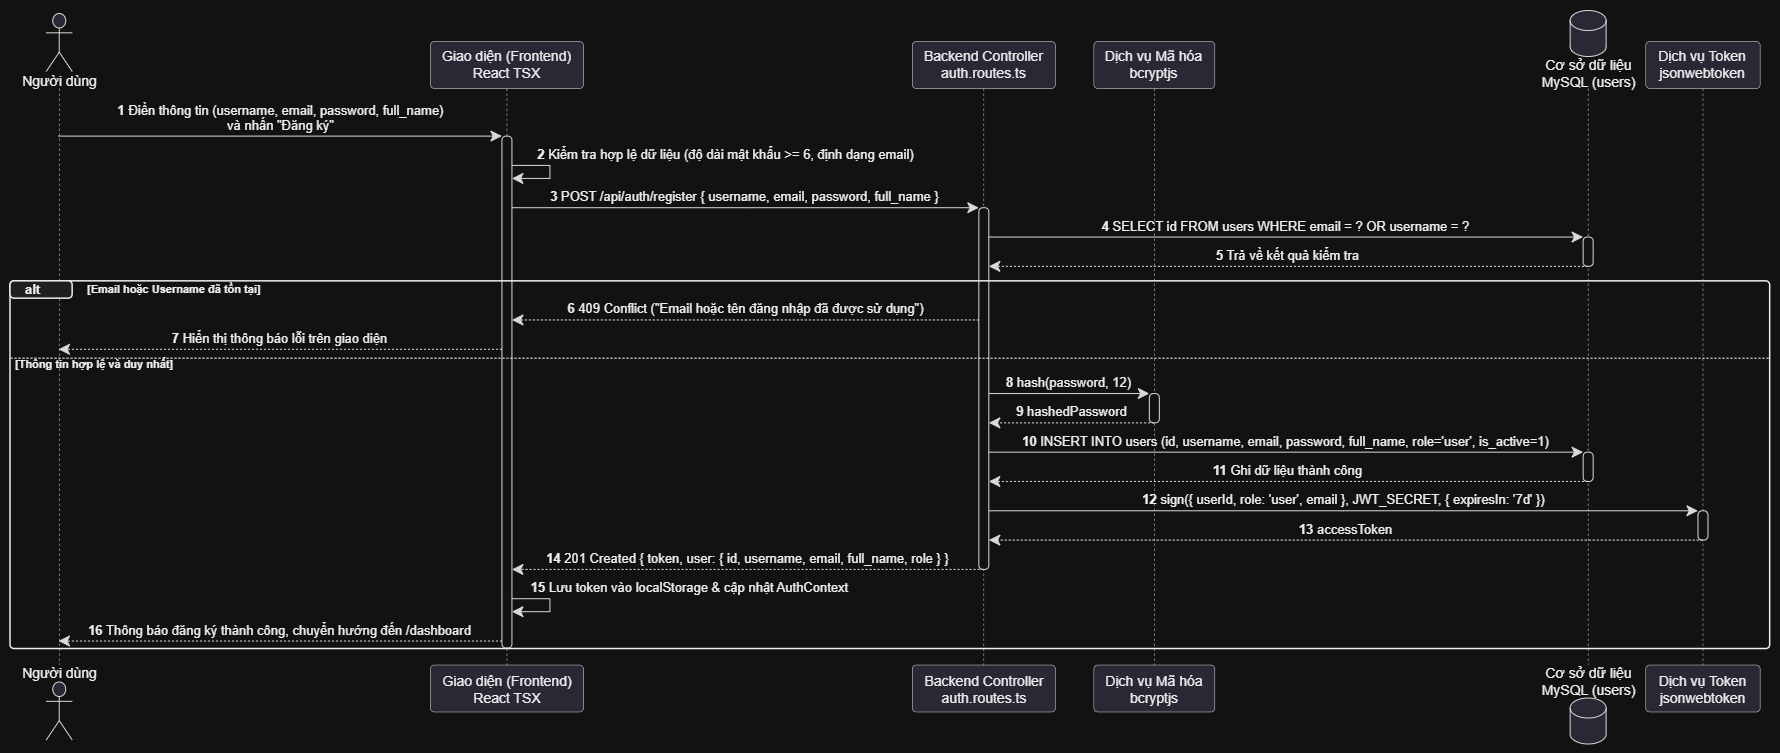
\includegraphics[width=0.94\textwidth]{figs/seq_dang_ky.png}
\caption{Sơ đồ tuần tự quy trình Đăng ký tài khoản người dùng mới.}
\label{fig:seq_dang_ky}
\end{figure}

\noindent\textbf{Mô tả:} Hình~\ref{fig:seq_dang_ky} mô tả sơ đồ tuần tự quy trình đăng ký tài khoản mới giữa Người dùng, Giao diện RegisterPage, Bộ điều khiển AuthController, Thư viện BCrypt và Cơ sở dữ liệu MySQL (bảng users). Luồng tương tác bao gồm: nhập dữ liệu, kiểm tra định dạng tại client, gửi yêu cầu POST /api/auth/register, truy vấn kiểm tra trùng lặp email/username, băm mật khẩu và lưu hồ sơ tài khoản mới.

\noindent\textbf{Diễn giải:} Quy trình này thiết lập cơ chế xác thực hai lớp nghiêm ngặt nhằm bảo vệ an toàn thông tin. Kiểm tra Regex phía client giúp người dùng nhận phản hồi tức thời về định dạng hợp lệ. Ở tầng server, thao tác kiểm tra tính duy nhất giúp loại trừ hoàn toàn nguy cơ trùng lặp danh tính, và việc băm mật khẩu bằng BCrypt với salt rounds = 12 đảm bảo dữ liệu đăng nhập không bao giờ bị lưu dưới dạng văn bản thô (plain text), triệt tiêu rủi ro lộ lọt thông tin.

\subsubsection{2. Sơ đồ tuần tự Đăng nhập và Phân quyền người dùng}

Quy trình xác thực đăng nhập và bảo vệ phiên làm việc dựa trên mã chứng thực JSON Web Token (JWT) được thể hiện tại Hình~\ref{fig:seq_dang_nhap}:
\begin{enumerate}[leftmargin=1.6em, itemsep=2pt]
  \item Người dùng nhập email và mật khẩu tại trang đăng nhập, nhấn nút \en{``Đăng nhập''}.
  \item Frontend kiểm tra tính hợp lệ cơ bản của dữ liệu và gửi yêu cầu \code{POST /api/auth/login}.
  \item \code{Auth Controller} truy vấn bảng \code{users} theo địa chỉ email đã cung cấp.
  \item Nếu không tìm thấy tài khoản, trả về mã lỗi \code{HTTP 401 Unauthorized}. Nếu tìm thấy, kiểm tra cờ trạng thái \code{is\_active}: nếu tài khoản đang bị khóa (giá trị 0), hệ thống chặn đăng nhập và trả về thông báo lỗi tài khoản bị vô hiệu hóa.
  \item Nếu tài khoản đang hoạt động, gọi hàm \code{bcrypt.compare()} để so khớp mật khẩu người dùng nhập với chuỗi băm lưu trữ trong CSDL.
  \item Khi xác thực thành công, hệ thống sử dụng bí mật \code{JWT\_SECRET} để ký số tạo mã chứng thực \code{JWT token} có thời hạn 7 ngày, chứa định danh \code{userId} và vai trò \code{role}.
  \item Trả về mã phản hồi \code{HTTP 200 OK} kèm token và thông tin hồ sơ người dùng.
  \item Frontend lưu JWT vào \code{localStorage}, cập nhật trạng thái toàn cục trong \code{AuthContext}.
  \item Dựa trên trường \code{role}, hệ thống tự động phân luồng điều hướng: nếu là Quản trị viên (\code{admin}) chuyển sang bảng điều khiển \code{/admin}; nếu là Khách hàng (\code{user}) chuyển sang trang chủ \code{/dashboard}.
\end{enumerate}

\begin{figure}[H]
\centering
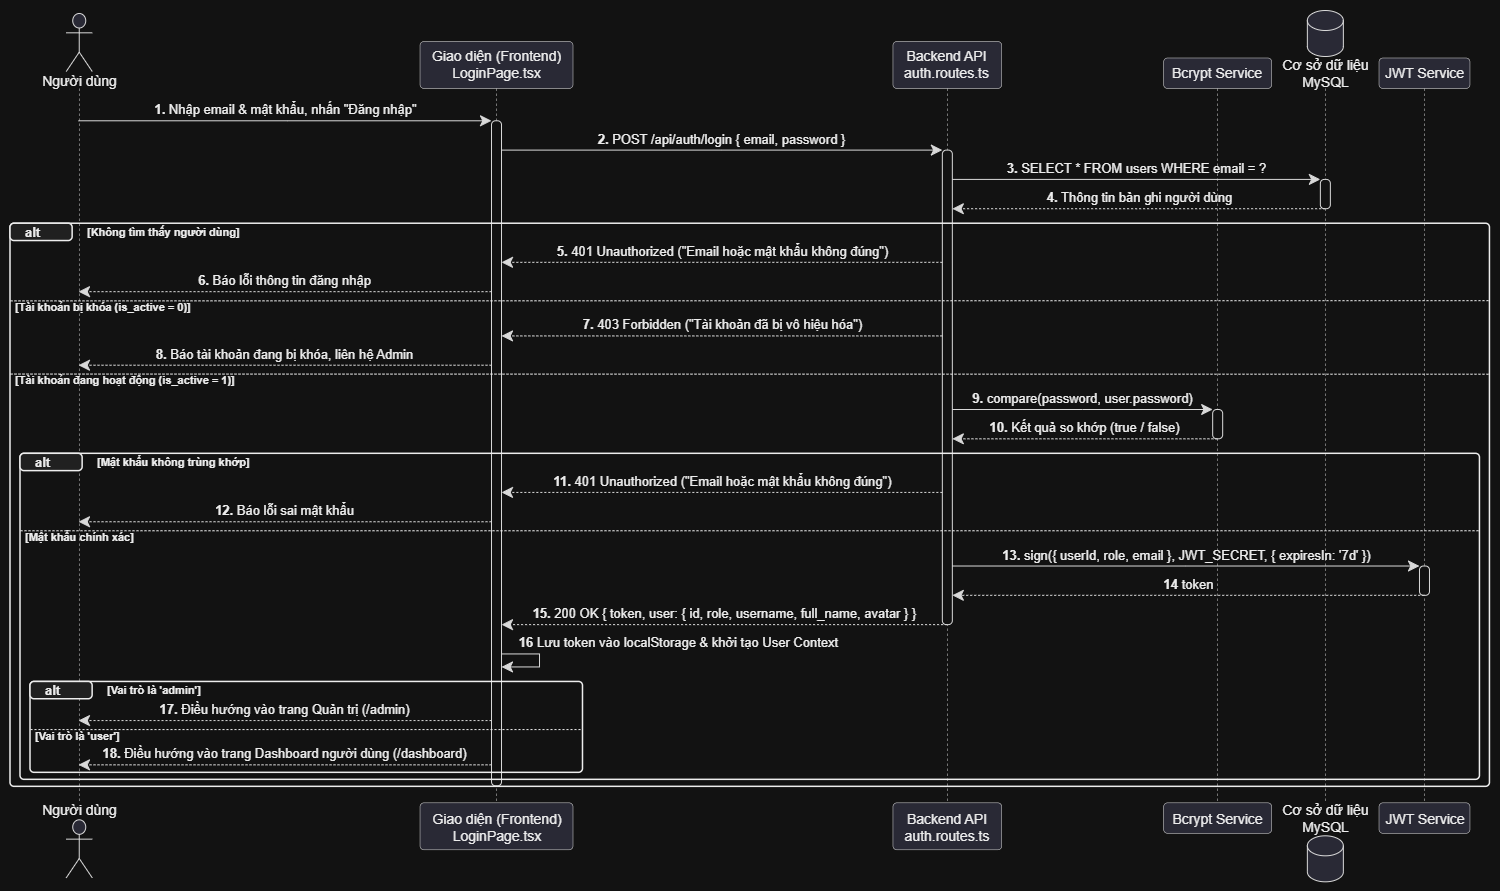
\includegraphics[width=0.96\textwidth]{figs/seq_dang_nhap.png}
\caption{Sơ đồ tuần tự quy trình Đăng nhập và Phân quyền người dùng (JWT).}
\label{fig:seq_dang_nhap}
\end{figure}

\noindent\textbf{Mô tả:} Hình~\ref{fig:seq_dang_nhap} mô tả sơ đồ tuần tự quy trình đăng nhập và phân quyền truy cập gồm các tác tử và đối tượng: Người dùng, LoginPage, AuthController, BCrypt, MySQL (users table) và AuthContext. Các bước thể hiện tuần tự từ khâu gửi thông tin đăng nhập, xác minh sự tồn tại của tài khoản, kiểm tra trạng thái hoạt động (is\_active), so khớp băm mật khẩu, ký tạo JWT token đến lưu trữ phiên làm việc và phân luồng điều hướng theo vai trò.

\noindent\textbf{Diễn giải:} Sơ đồ làm rõ cách thức hệ thống áp dụng giao thức xác thực phi trạng thái (Stateless Authentication) qua JWT. Việc kiểm tra trường is\_active trước khi so sánh mật khẩu giúp ngăn chặn kịp thời các tài khoản đã bị quản trị viên đình chỉ hoạt động. Token được ký bảo mật chứa mã người dùng và quyền hạn (role) cho phép phía Client nhận biết ngay quyền của người dùng để điều hướng chuẩn xác sang giao diện phù hợp (Dashboard cho User hoặc Admin Panel cho Quản trị viên), đồng thời bảo vệ các API nghiệp vụ tiếp theo không bị truy cập trái phép.

\subsubsection{3. Sơ đồ tuần tự Gợi ý món ăn thông minh Hybrid}

Quy trình gợi ý món ăn thông minh là chức năng hạt nhân của hệ thống FoodAI, tích hợp mô hình ngôn ngữ lớn Google Gemini AI cùng cơ chế phòng vệ dự phòng Fallback khi mất mạng (Hình~\ref{fig:seq_goi_y_mon_an}):
\begin{enumerate}[leftmargin=1.6em, itemsep=2pt]
  \item Người dùng nhập danh sách nguyên liệu hoặc chọn nhanh từ các bộ combo gợi ý, nhấn nút \en{``Gợi ý món ăn''}.
  \item Frontend gửi yêu cầu \code{POST /api/recipes/suggest} đính kèm danh sách nguyên liệu và mã Bearer JWT token.
  \item \code{Recipe Controller} xác thực token qua middleware, đồng thời kích hoạt bộ kiểm soát tần suất \en{Rate Limiting} (tối đa 20 yêu cầu/phút) để ngăn chặn hành vi tấn công từ chối dịch vụ.
  \item Hệ thống bất đồng bộ lưu vết danh sách nguyên liệu vào bảng \code{search\_history} phục vụ tính năng tái sử dụng và thống kê quản trị.
  \item \code{Recipe Controller} chuyển tiếp dữ liệu sang mô-đun \code{gemini.service.ts}.
  \item \code{Gemini Service} thiết lập Prompt kỹ thuật cao theo cấu trúc phân vai chuyên gia ẩm thực (\en{AI Chef \& Nutritionist}), kích hoạt chế độ ép kiểu dữ liệu \code{responseMimeType: 'application/json'} và áp dụng nghiêm ngặt quy tắc loại trừ cấm tự bịa thành phần đạm chính (thịt/cá lạ).
  \item Gửi Prompt tới đám mây Google Gemini thông qua thư viện \code{@google/generative-ai}.
\end{enumerate}

Luồng xử lý được rẽ nhánh linh hoạt theo hai kịch bản:
\begin{itemize}[leftmargin=1.6em, itemsep=2pt]
  \item \textbf{Kịch bản chính (Google Gemini phản hồi thành công):}
  \begin{itemize}
    \item Google Gemini trả về chuỗi văn bản JSON chứa danh sách 6 món ăn kèm mẹo nấu và 8 chỉ số dinh dưỡng.
    \item \code{Gemini Service} tiến hành làm sạch ký tự Markdown (\code{```json}), phân tích cú pháp chuỗi JSON, lọc khử trùng lặp và kích hoạt hàm \code{extractPrimaryIngredients} rà soát đạm lạ.
    \item Hệ thống gọi \code{Image Service} để truy vấn kho ảnh Cookpad từ bảng \code{cookpad\_dish\_images}, áp dụng thuật toán chấm điểm \code{scoreRecipeCard} nhằm loại bỏ các hình ảnh bento tạo hình hoặc đồ ăn dặm.
    \item Gán đường dẫn ảnh thực tế chất lượng cao độc nhất cho từng món gợi ý, đảm bảo không có hai món nào bị trùng ảnh trong cùng một phiên tìm kiếm.
    \item Trả về danh sách 6 món ăn hoàn chỉnh với cờ nguồn \code{source = 'ai'}.
  \end{itemize}
  \item \textbf{Kịch bản dự phòng (Sự cố mạng, Timeout hoặc vượt Quota):}
  \begin{itemize}
    \item Khi xảy ra lỗi kết nối bên thứ ba, khối \code{catch} bắt ngoại lệ và kích hoạt ngay hàm dự phòng \code{suggestRecipesFromDatabase()}.
    \item Truy vấn trực tiếp từ bảng \code{recipes} trong CSDL MySQL theo giải thuật so khớp Heuristic với ma trận nguyên liệu đồng nghĩa và ranh giới từ nguyên vẹn.
    \item Trả về danh sách món ăn từ kho Cookpad nội bộ với cờ nguồn \code{source = 'fallback'} mà không gây gián đoạn trải nghiệm người dùng.
  \end{itemize}
\end{itemize}

Frontend tiếp nhận kết quả phản hồi \code{HTTP 200 OK} và kết xuất danh sách Recipe Card trực quan ra màn hình.

\begin{figure}[H]
\centering
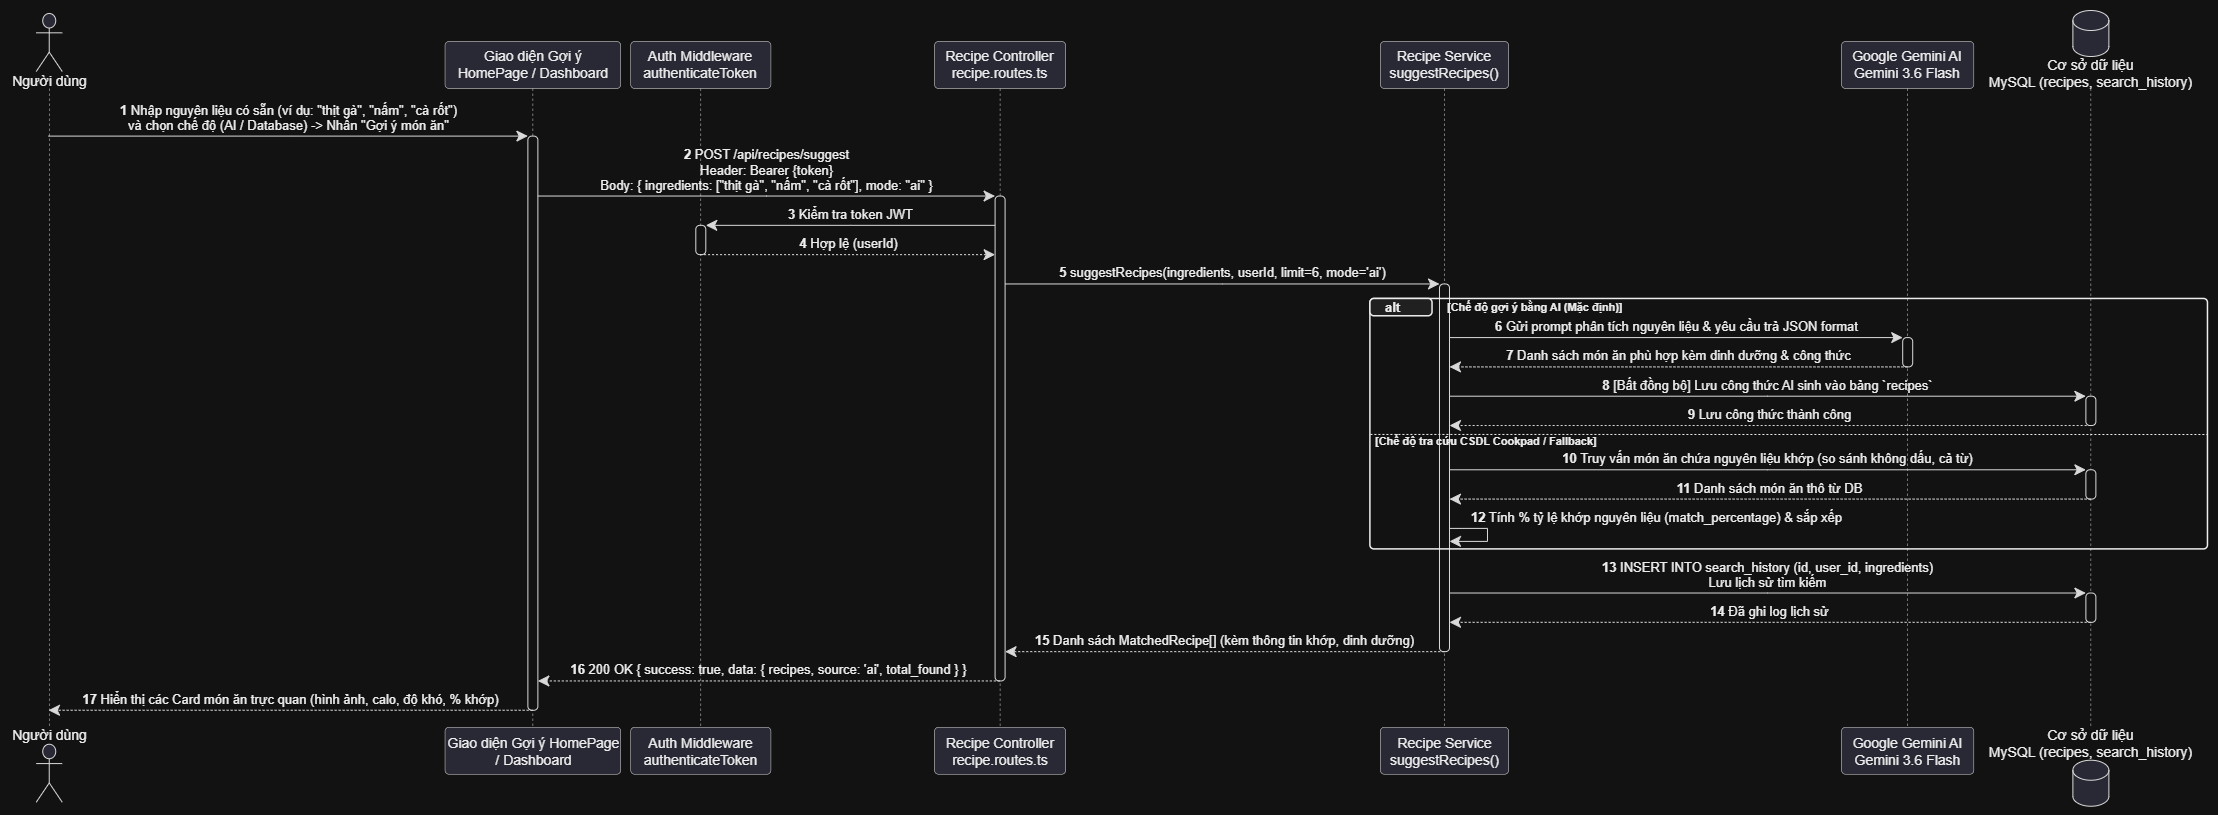
\includegraphics[width=\textwidth]{figs/seq_goi_y_mon_an.png}
\caption{Sơ đồ tuần tự quy trình Gợi ý món ăn thông minh Hybrid.}
\label{fig:seq_goi_y_mon_an}
\end{figure}

\noindent\textbf{Mô tả:} Hình~\ref{fig:seq_goi_y_mon_an} mô tả sơ đồ tuần tự quy trình gợi ý món ăn thông minh theo kiến trúc kết hợp (Hybrid) giữa Người dùng, Dashboard UI, RecipeController, GeminiService, ImageService và CSDL MySQL. Sơ đồ minh họa rành mạch hai nhánh xử lý: (1) Nhánh chính với Google Gemini AI khi có kết nối mạng và API Key hợp lệ, trải qua các bước làm sạch JSON, hậu kiểm loại trừ đạm lạ và gán ảnh Cookpad; (2) Nhánh dự phòng Fallback tự động kích hoạt khi AI gặp sự cố để truy xuất trực tiếp từ kho món ăn Cookpad MySQL nội bộ.

\noindent\textbf{Diễn giải:} Sơ đồ này chứng minh tính chịu lỗi (Fault-Tolerant) và độ sẵn sàng cao của hệ thống FoodAI. Việc kết hợp AI tạo sinh với quy tắc lọc ngữ nghĩa tiếng Việt nghiêm ngặt giải quyết triệt để vấn đề ảo giác nguyên liệu thịt cá mà các mô hình ngôn ngữ lớn thường gặp phải. Khi xảy ra sự cố mạng bên ngoài hoặc vượt định ngạch API, cơ chế Fallback nội bộ phản hồi ngay lập tức trong thời gian dưới 300ms, đảm bảo người dùng luôn nhận được gợi ý món ăn có liên quan mà trải nghiệm không bao giờ bị gián đoạn.

\subsubsection{4. Sơ đồ tuần tự Xem chi tiết công thức nấu và Phân tích dinh dưỡng}

Quy trình xem chi tiết công thức và thông tin vi chất hỗ trợ người dùng có được bức tranh toàn diện trước khi bắt tay vào chế biến (Hình~\ref{fig:seq_xem_chi_tiet_dinh_duong}):
\begin{enumerate}[leftmargin=1.6em, itemsep=2pt]
  \item Người dùng nhấn vào thẻ món ăn hoặc nút \en{``Xem chi tiết''} trên giao diện trang chủ.
  \item Frontend gửi yêu cầu trích xuất chi tiết công thức hoặc kích hoạt Modal 3 Tab tích hợp sẵn từ dữ liệu gợi ý.
  \item Nếu là món ăn chưa có đầy đủ hướng dẫn từng bước, hệ thống gửi yêu cầu \code{POST /api/recipes/ai-recipe-detail} kèm tên món ăn lên Backend.
  \item \code{Gemini Service} sinh bản phân tích chuyên sâu gồm: định lượng chính xác từng nguyên liệu (gam/ml), danh sách các bước nấu nướng tuần tự kèm thời gian chế biến, và bảng 8 chỉ số dinh dưỡng định lượng (năng lượng calo, protein, carbs, chất béo, chất xơ, vitamin C, canxi, sắt).
  \item Backend trả về đối tượng chi tiết cấu trúc JSON chuẩn về cho Frontend.
  \item Frontend hiển thị cửa sổ Modal tương tác với 3 phân hệ rành mạch: Tab 1 --- Định lượng nguyên liệu (đánh dấu xanh các nguyên liệu đã có); Tab 2 --- Hướng dẫn nấu ăn 4--6 bước rõ ràng; Tab 3 --- Bảng vi chất dinh dưỡng khoa học.
\end{enumerate}

\begin{figure}[H]
\centering
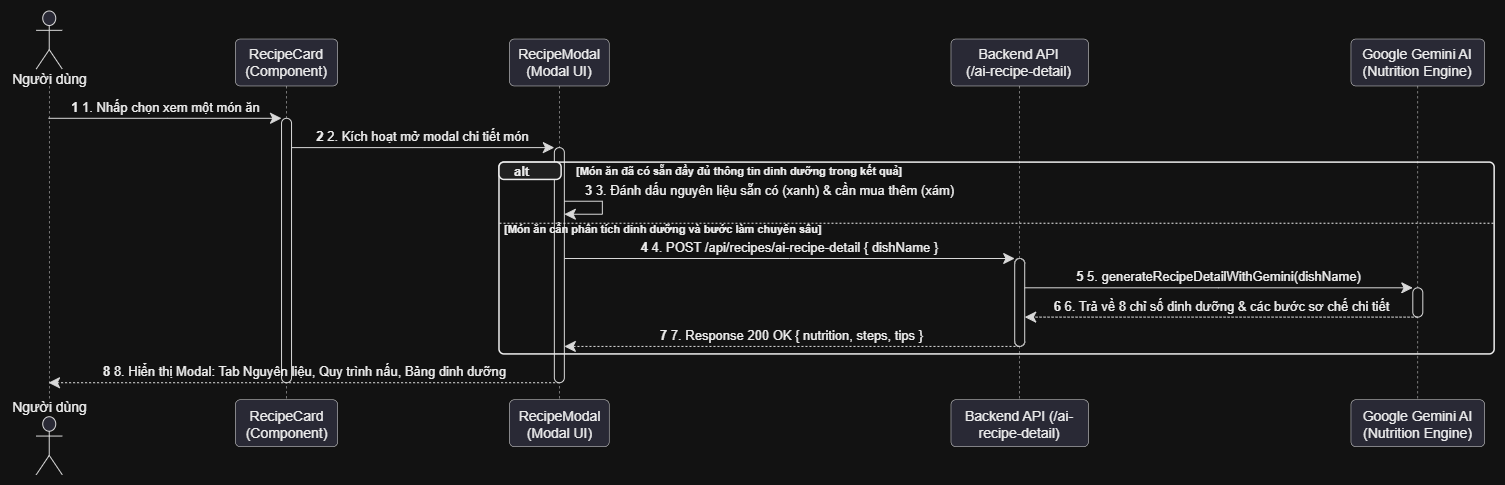
\includegraphics[width=0.94\textwidth]{figs/seq_xem_chi_tiet_dinh_duong.png}
\caption{Sơ đồ tuần tự quy trình Xem chi tiết công thức nấu và Phân tích dinh dưỡng.}
\label{fig:seq_xem_chi_tiet_dinh_duong}
\end{figure}

\noindent\textbf{Mô tả:} Hình~\ref{fig:seq_xem_chi_tiet_dinh_duong} mô tả sơ đồ tuần tự quy trình hiển thị chi tiết công thức và phân tích dinh dưỡng giữa Người dùng, RecipeCard/Modal, RecipeController, GeminiService và cơ sở dữ liệu. Luồng thực hiện gồm: kích hoạt xem chi tiết từ thẻ món, kiểm tra tính đầy đủ của dữ liệu công thức, gọi mô-đun AI làm giàu thêm thông tin nếu cần thiết, và kết xuất dữ liệu phân chia theo 3 tab chuyên biệt trên giao diện Modal.

\noindent\textbf{Diễn giải:} Quy trình này làm nổi bật năng lực chuyên gia ẩm thực (AI Chef) và chuyên gia dinh dưỡng của hệ thống. Thay vì chỉ cung cấp công thức nấu đơn thuần như các trang mạng truyền thống, việc tích hợp bảng 8 chỉ số vi chất dinh dưỡng (calo, protein, carbs, fat, xơ, vitamin C, canxi, sắt) giúp người dùng quản lý khẩu phần ăn khoa học. Thiết kế giao diện 3 Tab phân tách rõ nguyên liệu có sẵn và nguyên liệu cần chuẩn bị thêm, giúp người dùng dễ dàng lập kế hoạch nấu nướng.

\subsubsection{5. Sơ đồ tuần tự Quản lý và Lưu món ăn yêu thích}

Quy trình quản lý sổ tay ẩm thực cá nhân cho phép người dùng lưu lại những công thức yêu thích để nấu lại sau này (Hình~\ref{fig:seq_quan_ly_yeu_thich}):
\begin{enumerate}[leftmargin=1.6em, itemsep=2pt]
  \item Người dùng nhấn vào biểu tượng Trái tim trên Card món ăn hoặc bên trong Modal chi tiết.
  \item Giao diện gửi yêu cầu \code{POST /api/recipes/favorites} mang theo toàn bộ đối tượng dữ liệu món ăn dạng JSON cùng mã chứng thực Bearer JWT token.
  \item \code{Recipe Controller} giải mã token để trích xuất \code{userId} và kiểm tra tính hợp lệ của gói tin.
  \item Hệ thống thực thi câu lệnh \code{SELECT} trên bảng \code{favorite\_recipes} để kiểm tra xem món ăn này đã được người dùng lưu trước đó hay chưa (dựa theo \code{recipe\_id} hoặc tên món ăn).
  \item Nếu món ăn đã tồn tại, phản hồi mã lỗi \code{HTTP 409 Conflict} để tránh lưu trùng lặp.
  \item Nếu chưa tồn tại, hệ thống khởi tạo khóa chính UUID v4 và thực thi lệnh \code{INSERT INTO favorite\_recipes} lưu trữ toàn bộ dữ liệu công thức vào trường \code{recipe\_data}.
  \item Cơ sở dữ liệu xác nhận ghi dữ liệu thành công, phản hồi mã trạng thái \code{HTTP 200 OK}.
  \item Frontend chuyển trạng thái icon trái tim sang màu đỏ kích hoạt \en{(Active State)}, đồng thời hiển thị thông báo Toast xác nhận: \en{``Đã thêm vào danh sách yêu thích''}.
\end{enumerate}

\begin{figure}[H]
\centering
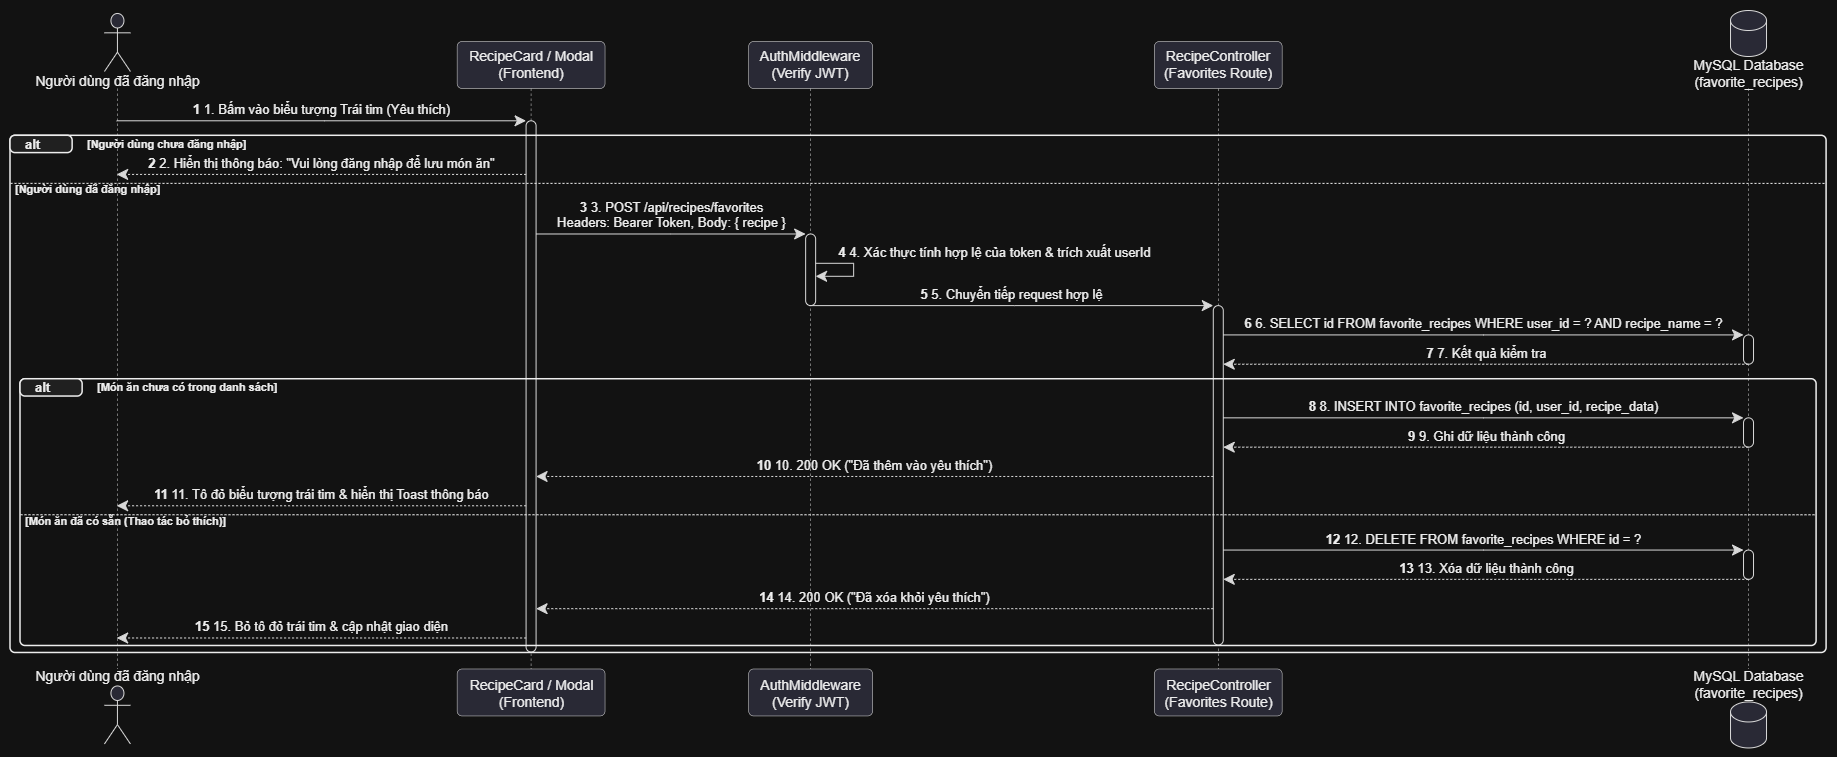
\includegraphics[width=0.94\textwidth]{figs/seq_quan_ly_yeu_thich.png}
\caption{Sơ đồ tuần tự quy trình Quản lý và Lưu món ăn yêu thích.}
\label{fig:seq_quan_ly_yeu_thich}
\end{figure}

\noindent\textbf{Mô tả:} Hình~\ref{fig:seq_quan_ly_yeu_thich} mô tả sơ đồ tuần tự lưu trữ món ăn yêu thích của người dùng, liên kết tương tác giữa Người dùng, Nút biểu tượng Trái tim, RecipeController, Middleware JWT và bảng favorite\_recipes trong MySQL. Trình tự bao gồm: nhấn icon yêu thích, kiểm tra phiên đăng nhập bằng JWT, kiểm tra trùng lặp bản ghi trong cơ sở dữ liệu, chèn bản ghi JSON công thức mới và cập nhật trạng thái hiển thị của icon trên giao diện.

\noindent\textbf{Diễn giải:} Sơ đồ thể hiện kỹ thuật quản lý dữ liệu cá nhân hóa an toàn. Việc liên kết món ăn yêu thích với định danh userId lấy trực tiếp từ JWT ngăn chặn hoàn toàn việc người dùng can thiệp vào bộ sưu tập của người khác. Cơ chế kiểm tra trùng lặp trước khi thực hiện lệnh INSERT giúp cơ sở dữ liệu duy trì tính toàn vẹn, tránh lãng phí dung lượng lưu trữ và ngăn ngừa xung đột dữ liệu khi người dùng vô tình bấm nhiều lần liên tiếp.

\subsubsection{6. Sơ đồ tuần tự Quản trị tài khoản người dùng}

Phân hệ quản trị dành riêng cho Quản trị viên (\code{Admin}) để quản lý vòng đời tài khoản người dùng và giám sát hệ thống (Hình~\ref{fig:seq_quan_tri_nguoi_dung}):
\begin{enumerate}[leftmargin=1.6em, itemsep=2pt]
  \item Quản trị viên đăng nhập với tài khoản Admin và truy cập vào đường dẫn quản trị người dùng \code{/admin/users}.
  \item Frontend gửi yêu cầu \code{GET /api/admin/users} có đính kèm Bearer token tới máy chủ.
  \item Middleware \code{authenticateToken} và bộ lọc phân quyền \code{requireAdmin} kiểm tra tính hợp lệ của token và xác minh vai trò \code{role === 'admin'}. Nếu không phải admin, hệ thống từ chối truy cập với mã lỗi \code{HTTP 403 Forbidden}.
  \item Khi xác thực thành công, \code{Admin Controller} thực thi truy vấn lấy danh sách toàn bộ người dùng có phân trang (10 bản ghi/trang), kèm thông tin tổng hợp số lượt tìm kiếm và số món ăn đã lưu.
  \item CSDL MySQL trả về tập dữ liệu, máy chủ gửi phản hồi \code{HTTP 200 OK} về Frontend để kết xuất bảng dữ liệu trực quan.
  \item Khi Quản trị viên thực hiện thao tác thay đổi trạng thái (Kích hoạt/Vô hiệu hóa tài khoản) hoặc Đặt lại mật khẩu:
  \begin{itemize}
    \item Frontend gửi yêu cầu \code{PUT /api/admin/users/:id/status} hoặc \code{PUT /api/admin/users/:id/reset-password}.
    \item Hệ thống kiểm tra quy tắc an toàn cốt lõi: Quản trị viên tuyệt đối không thể tự khóa hoặc tự xóa tài khoản của chính mình.
    \item \code{Admin Controller} thực thi cập nhật bản ghi trong bảng \code{users} và phản hồi thông báo thành công.
    \item Frontend cập nhật trạng thái bảng dữ liệu theo thời gian thực (Real-time UI Update) và hiển thị thông báo Toast.
  \end{itemize}
\end{enumerate}

\begin{figure}[H]
\centering
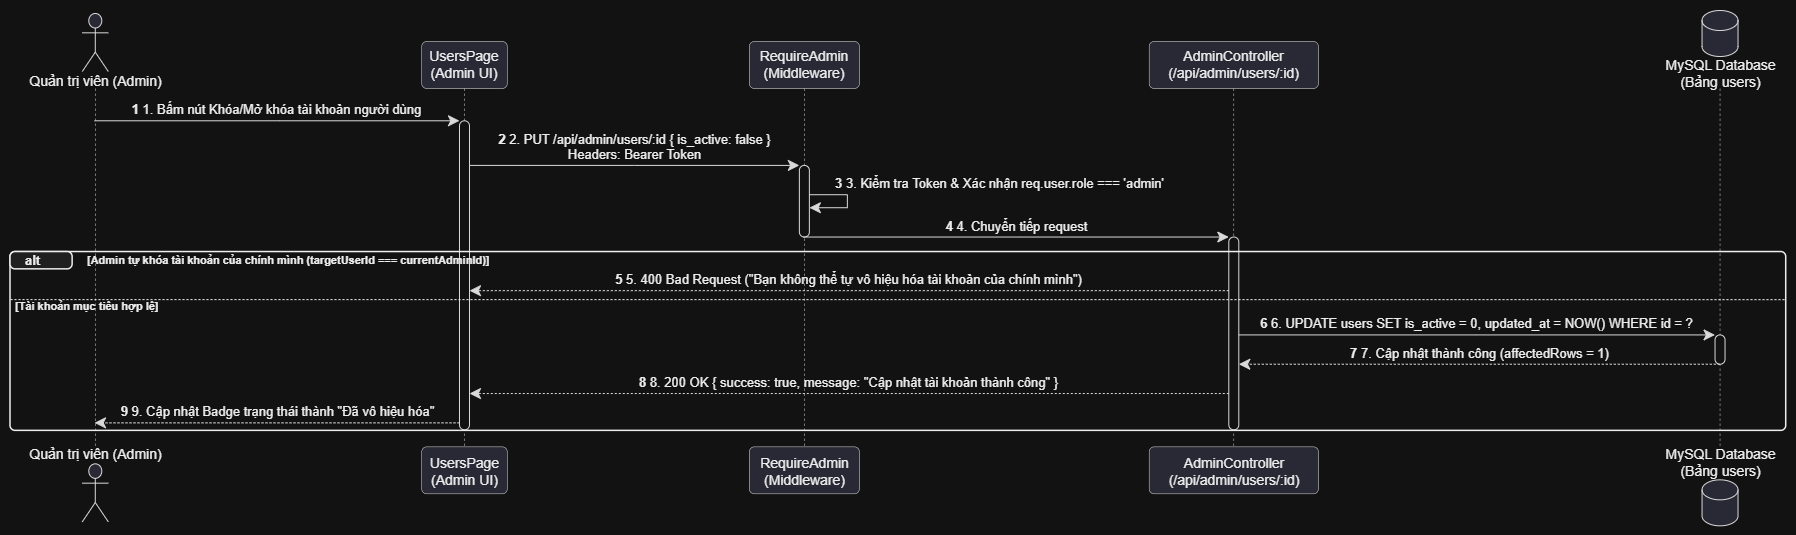
\includegraphics[width=0.94\textwidth]{figs/seq_quan_tri_nguoi_dung.png}
\caption{Sơ đồ tuần tự quy trình Quản trị tài khoản người dùng.}
\label{fig:seq_quan_tri_nguoi_dung}
\end{figure}

\noindent\textbf{Mô tả:} Hình~\ref{fig:seq_quan_tri_nguoi_dung} mô tả sơ đồ tuần tự các thao tác quản trị tài khoản người dùng, bao gồm: Quản trị viên, Trang AdminUsersPage, Bộ kiểm soát phân quyền requireAdmin Middleware, AdminController và bảng users trong CSDL MySQL. Sơ đồ biểu diễn hai luồng chính: tải danh sách tài khoản phân trang kèm số liệu thống kê và thực hiện cập nhật trạng thái kích hoạt/khóa tài khoản hoặc đặt lại mật khẩu.

\noindent\textbf{Diễn giải:} Sơ đồ làm rõ tầng phòng thủ bảo mật cấp cao nhất của hệ thống. Bộ lọc requireAdmin chặn đứng từ cửa ngõ các yêu cầu giả mạo từ người dùng thông thường bằng mã lỗi HTTP 403 Forbidden. Điểm đặc biệt quan trọng trong nghiệp vụ là cơ chế kiểm tra an toàn tại server: ngăn chặn tuyệt đối tình huống Quản trị viên tự khóa tài khoản của chính mình, đảm bảo hệ thống luôn luôn có ít nhất một tài khoản Admin đang hoạt động để duy trì quyền điều hành.

\section{Thiết kế kiến trúc hệ thống}

Hệ thống được thiết kế theo mô hình kiến trúc ba tầng \en{(Three-Tier Architecture)} hiện đại, đảm bảo tính mô-đun hóa, bảo mật và khả năng mở rộng dễ dàng (Hình~\ref{fig:kientruc_hethong}).

\begin{figure}[H]
\centering
\resizebox{\textwidth}{!}{%
\begin{tikzpicture}[node distance=10mm and 12mm]
  % Tầng Client
  \node[startstop, fill=lightnavy, draw=daunavy] (client) {\textbf{TẦNG GIAO DIỆN (CLIENT LAYER)}\\React 18 + TypeScript + Vite + Tailwind CSS\\(User Dashboard \& Admin Dashboard)};

  % Tầng Server
  \node[process, fill=white, draw=daumaroon, below=12mm of client] (server) {\textbf{TẦNG ỨNG DỤNG (SERVER LAYER)}\\Node.js + Express RESTful API\\Auth Middleware (JWT) $\cdot$ Rate Limiter $\cdot$ CORS};

  % Khối dịch vụ bên trong Server
  \node[clsbox, below left=10mm and -5mm of server] (ai_svc) {Gemini Service\\(AI Chef \& Nutritionist)};
  \node[clsbox, below=10mm of server] (recipe_svc) {Recipe Service\\(Heuristic Matching)};
  \node[clsbox, below right=10mm and -5mm of server] (img_svc) {Image Service\\(Multi-source Retrieval)};

  % Tầng Dữ liệu & AI bên ngoài
  \node[objbox, below=14mm of recipe_svc] (db) {\textbf{CƠ SỞ DỮ LIỆU}\\MySQL 8.0 / SQLite\\(Users, Recipes, Cookpad Images, Favorites, History)};

  \node[membox, left=10mm of db] (gemini_ext) {\textbf{Google Gemini API}\\(LLM Engine)};
  \node[membox, right=10mm of db] (pexels_ext) {\textbf{Pexels \& Cookpad}\\(Image Sources)};

  % Kết nối
  \draw[flowarr] (client) -- node[right, font=\tiny]{HTTPS / JSON} (server);
  \draw[flowarr] (server) -- (ai_svc);
  \draw[flowarr] (server) -- (recipe_svc);
  \draw[flowarr] (server) -- (img_svc);
  \draw[flowarr] (ai_svc) -- (gemini_ext);
  \draw[flowarr] (recipe_svc) -- (db);
  \draw[flowarr] (img_svc) -- (pexels_ext);
  \draw[flowarr] (img_svc) -- (db);
\end{tikzpicture}}
\caption{Sơ đồ kiến trúc phân tầng tổng thể của hệ thống FoodAI.}
\label{fig:kientruc_hethong}
\end{figure}

\noindent\textbf{Mô tả:} Hình~\ref{fig:kientruc_hethong} mô tả kiến trúc phân tầng tổng thể của hệ thống FoodAI theo mô hình 3 tầng (Three-Tier Architecture), bao gồm: (1) Tầng giao diện Client Layer (React 18, TypeScript, Vite, Tailwind CSS); (2) Tầng ứng dụng Server Layer (Node.js, Express RESTful API với các khối Auth Middleware, Rate Limiter, Gemini Service, Recipe Service, Image Service); và (3) Tầng dữ liệu \& dịch vụ bên ngoài (CSDL MySQL 8.0, Google Gemini API, Pexels API và kho ảnh Cookpad).

\noindent\textbf{Diễn giải:} Sơ đồ thể hiện tính phân tách trách nhiệm (Separation of Concerns) cao giữa các tầng. Mọi yêu cầu từ Client đều phải thông qua giao thức HTTPS có kiểm soát bởi Middleware xác thực và giới hạn tần suất (Rate Limiter) trước khi chạm tới các dịch vụ nghiệp vụ. Việc bóc tách các Service độc lập (Gemini Service cho AI, Recipe Service cho giải thuật so khớp, Image Service cho truy xuất ảnh) giúp mã nguồn đạt độ gắn kết cao, giảm thiểu phụ thuộc lỏng lẻo, tạo điều kiện thuận lợi cho việc kiểm thử đơn vị, bảo trì và mở rộng tính năng mà không gây ảnh hưởng tới toàn bộ hệ thống.

\section{Thiết kế cơ sở dữ liệu}

Cơ sở dữ liệu quan hệ của hệ thống được thiết kế chuẩn hóa để lưu trữ thông tin người dùng, công thức ẩm thực, hình ảnh cào từ Cookpad và dữ liệu tương tác (Bảng~\ref{tab:schema_users} và Bảng~\ref{tab:schema_recipes}).

\begin{table}[H]
\centering
\caption{Lược đồ cấu trúc bảng người dùng (\code{users}).}
\label{tab:schema_users}
\begin{tabularx}{\textwidth}{@{}>{\bfseries\color{daunavy}}p{2.6cm} >{\color{daumaroon}}p{2.8cm} >{\raggedright\arraybackslash}X@{}}
\toprule
\rowcolor{gray100}\bfseries\color{daunavy}Tên cột & \bfseries\color{daumaroon}Kiểu dữ liệu & \bfseries\color{daunavy}Ràng buộc \& Ý nghĩa \\
\midrule
id          & VARCHAR(36)  & Khóa chính (UUID v4) \\
username    & VARCHAR(50)  & Tên đăng nhập duy nhất (UNIQUE, NOT NULL) \\
email       & VARCHAR(100) & Địa chỉ email duy nhất (UNIQUE, NOT NULL) \\
password    & VARCHAR(255) & Mật khẩu đã băm (Bcrypt hash) \\
full\_name  & VARCHAR(100) & Họ và tên hiển thị \\
role        & VARCHAR(10)  & Vai trò tài khoản (\code{'user'} hoặc \code{'admin'}) \\
is\_active  & TINYINT(1)   & Trạng thái kích hoạt tài khoản (1: Hoạt động, 0: Khóa) \\
created\_at & DATETIME     & Thời điểm tạo tài khoản \\
\bottomrule
\end{tabularx}
\end{table}

\noindent\textbf{Mô tả:} Bảng~\ref{tab:schema_users} mô tả chi tiết lược đồ cấu trúc của bảng \code{users} gồm 8 trường dữ liệu: id (khóa chính UUID), username (tên đăng nhập duy nhất), email (địa chỉ thư điện tử duy nhất), password (chuỗi băm BCrypt 255 ký tự), full\_name (họ tên hiển thị), role (vai trò người dùng), is\_active (cờ trạng thái kích hoạt) và created\_at (mốc thời gian tạo tài khoản).

\noindent\textbf{Diễn giải:} Thiết kế bảng đáp ứng chuẩn dạng chuẩn 3 (3NF) trong cơ sở dữ liệu quan hệ. Ràng buộc UNIQUE trên hai trường username và email ngăn chặn tuyệt đối tình trạng đăng ký trùng lặp tài khoản. Việc lưu trữ mật khẩu bằng chuỗi băm BCrypt 255 ký tự đảm bảo an toàn tối đa theo các tiêu chuẩn an ninh mạng hiện đại. Trường cờ is\_active cho phép quản trị viên có thể vô hiệu hóa quyền truy cập của tài khoản vi phạm chính sách một cách linh hoạt mà vẫn bảo toàn toàn bộ dữ liệu lịch sử tìm kiếm và món ăn yêu thích liên kết.

\begin{table}[H]
\centering
\caption{Lược đồ cấu trúc bảng món ăn nội bộ (\code{recipes}).}
\label{tab:schema_recipes}
\begin{tabularx}{\textwidth}{@{}>{\bfseries\color{daunavy}}p{2.8cm} >{\color{daumaroon}}p{2.8cm} >{\raggedright\arraybackslash}X@{}}
\toprule
\rowcolor{gray100}\bfseries\color{daunavy}Tên cột & \bfseries\color{daumaroon}Kiểu dữ liệu & \bfseries\color{daunavy}Ràng buộc \& Ý nghĩa \\
\midrule
id            & VARCHAR(36)  & Khóa chính món ăn \\
name          & VARCHAR(255) & Tên món ăn tiếng Việt (INDEX) \\
description   & TEXT         & Mô tả vắn tắt về hương vị \\
image\_url    & VARCHAR(1000)& Đường dẫn ảnh món ăn thực tế \\
cooking\_time & INT          & Thời gian chế biến (phút) \\
difficulty    & VARCHAR(20)  & Độ khó (\code{'Dễ'}, \code{'Trung bình'}, \code{'Khó'}) \\
category      & VARCHAR(50)  & Danh mục (\code{'Món xào'}, \code{'Súp/Canh'}, \dots) \\
author\_name  & VARCHAR(100) & Tác giả chia sẻ công thức trên Cookpad \\
\bottomrule
\end{tabularx}
\end{table}

\noindent\textbf{Mô tả:} Bảng~\ref{tab:schema_recipes} mô tả cấu trúc bảng lưu trữ món ăn \code{recipes} với 8 thuộc tính nòng cốt: id (khóa chính), name (tên món ăn tiếng Việt có đánh chỉ mục INDEX), description (mô tả hương vị), image\_url (đường dẫn hình ảnh CDN), cooking\_time (thời gian nấu ước tính tính theo phút), difficulty (độ khó chế biến), category (danh mục phân loại) và author\_name (tác giả chia sẻ công thức).

\noindent\textbf{Diễn giải:} Bảng \code{recipes} đóng vai trò là cơ sở tri thức ẩm thực nội bộ (Internal Knowledge Base) của hệ thống. Việc đánh chỉ mục INDEX trên trường tên món ăn \code{name} giúp tối ưu hóa đáng kể tốc độ tìm kiếm văn bản và so khớp Heuristic khi hệ thống hoạt động ở chế độ Fallback, giảm thời gian phản hồi từ CSDL xuống dưới mức 50ms. Các trường định lượng như thời gian nấu và mức độ khó cung cấp siêu dữ liệu đầy đủ để giao diện người dùng hiển thị thẻ món ăn trực quan và hỗ trợ bộ lọc đa chiều.

Ngoài ra, hệ thống lưu trữ ảnh trích xuất trong bảng \code{cookpad\_dish\_images}, lưu trữ lịch sử người dùng trong \code{search\_history} và lưu công thức yêu thích dạng JSON chi tiết trong \code{favorite\_recipes}.

\section{Thiết kế thuật toán gợi ý và Xử lý ảnh thông minh}

\subsection{Luồng thực thi gợi ý món ăn thông minh}

Quy trình gợi ý món ăn kết hợp AI và Fallback được mô tả chi tiết tại Hình~\ref{fig:flow_suggest}.

\begin{figure}[H]
\centering
\resizebox{0.82\textwidth}{!}{%
\begin{tikzpicture}[node distance=10mm]
  \node[startstop] (start) {Bắt đầu: Tiếp nhận danh sách nguyên liệu $U$};
  \node[decision, below=8mm of start] (check_key) {Cấu hình Gemini API hợp lệ?};
  \node[process, below left=10mm and 2mm of check_key] (call_ai) {Gọi Google Gemini AI\\với Prompt ràng buộc};
  \node[decision, below=8mm of call_ai] (check_ai) {AI phản hồi \&\\Parse JSON thành công?};
  \node[process, below=8mm of check_ai] (post_filter) {Hậu kiểm: Khử trùng lặp\\và lọc vi phạm thịt cá};
  \node[process, right=20mm of check_ai] (fallback_db) {Kích hoạt chế độ Fallback:\\Tra cứu kho Cookpad MySQL};
  \node[process, below=8mm of post_filter] (attach_img) {Truy xuất \& Gán hình ảnh độc nhất\\từ Cookpad / Pexels / HD Bank};
  \node[startstop, below=8mm of attach_img] (finish) {Trả về danh sách 4--6 món ăn kèm\\công thức, dinh dưỡng và ảnh cho người dùng};

  \draw[flowarr] (start) -- (check_key);
  \draw[flowarr] (check_key) -| node[above, font=\footnotesize]{Có} (call_ai);
  \draw[flowarr] (check_key) -| node[above, font=\footnotesize]{Không} (fallback_db);
  \draw[flowarr] (call_ai) -- (check_ai);
  \draw[flowarr] (check_ai) -- node[right, font=\footnotesize]{Thành công} (post_filter);
  \draw[flowarr] (check_ai) -- node[above, font=\footnotesize]{Lỗi / Timeout} (fallback_db);
  \draw[flowarr] (fallback_db) |- (attach_img);
  \draw[flowarr] (post_filter) -- (attach_img);
  \draw[flowarr] (attach_img) -- (finish);
\end{tikzpicture}}
\caption{Sơ đồ khối luồng xử lý gợi ý món ăn thông minh (Hybrid Flowchart).}
\label{fig:flow_suggest}
\end{figure}

\noindent\textbf{Mô tả:} Hình~\ref{fig:flow_suggest} mô tả sơ đồ lưu đồ (Flowchart) tiến trình xử lý gợi ý món ăn, thể hiện các khối quyết định rẽ nhánh logic từ lúc tiếp nhận danh sách nguyên liệu đầu vào, kiểm tra điều kiện khả dụng của API Key, gọi mô hình Gemini AI, kiểm tra tính hợp lệ của gói tin JSON, tiến hành lọc khử vi phạm nguyên liệu, cơ chế kích hoạt nhánh Fallback cơ sở dữ liệu khi phát sinh lỗi, đến công đoạn gắn hình ảnh và trả về kết quả cuối cùng.

\noindent\textbf{Diễn giải:} Sơ đồ khối giải thích nguyên nhân hệ thống duy trì được tính ổn định và tính chính xác cao. Nhánh xử lý AI được kiểm soát chặt chẽ bởi hai chốt chặn: khối kiểm tra cú pháp JSON đảm bảo cấu trúc dữ liệu không bị gãy vỡ, và khối hậu kiểm ngữ nghĩa loại bỏ ngay các món ăn tự bịa thịt cá vi phạm ràng buộc nguyên liệu đầu vào. Nhánh rẽ Fallback sang kho Cookpad MySQL giải thích vì sao khi mất kết nối mạng hay hết quota Gemini, hệ thống vẫn trả về được các món ăn truyền thống chuẩn vị và có sẵn ảnh chất lượng cao mà không hiển thị màn hình trắng hay báo lỗi khó chịu cho người dùng.

\subsection{Giải thuật gợi ý món ăn theo kiến trúc Database-First RAG (Mã giả)}

Giải thuật gợi ý món ăn áp dụng kỹ thuật RAG định hướng CSDL (\en{Database-First Retrieval-Augmented Generation})~\cite{Lewis2020RAG} kết hợp làm giàu dữ liệu tự động bằng Google Gemini AI được đặc tả chi tiết tại Giải thuật~\ref{alg:hybrid_suggest}.

\begin{algorithm}[H]
\caption{Gợi ý món ăn thông minh Database-First RAG và AI Enrichment}
\label{alg:hybrid_suggest}
\begin{algorithmic}[1]
\Require Danh sách nguyên liệu người dùng $U$, số lượng món cần lấy $K = 8$
\Ensure Danh sách $R$ gồm các món ăn có tên, hình ảnh chuẩn MySQL, công thức và dinh dưỡng do AI phân tích
\State Khởi tạo danh sách kết quả $R \gets \emptyset$
\State \Comment{Bước 1: Truy vấn CSDL lọc món ăn thực tế và ảnh Cookpad theo logic nguyên liệu}
\State $Cand \gets$ \Call{SuggestRecipesFromDatabase}{$U$, $\max(2K, 10)$}
\If{\Call{IsGeminiEnabled}{} = \textbf{True}}
    \State \textbf{thử thực hiện (try):}
        \State \quad \Comment{Bước 2: Gửi danh sách món từ CSDL cho Gemini AI phân tích chuyên sâu}
        \State \quad $TargetDishes \gets Cand[0 \dots K-1]$
        \State \quad $P \gets$ \Call{BuildEnrichmentPrompt}{$U$, $TargetDishes$}
        \State \quad $RawResponse \gets$ \Call{GeminiGenerate}{$P$}
        \State \quad $ParsedDishes \gets$ \Call{ParseAndSanitizeJSON}{$RawResponse$}
        \State \quad $EnrichedRecipes \gets$ \Call{AlignWithDatabaseCandidates}{$ParsedDishes$, $TargetDishes$}
        \State \quad \Comment{Bước 3: Tự động đồng bộ và lưu công thức, dinh dưỡng AI về lại MySQL}
        \State \quad \Call{SaveAiRecipesToDatabase}{$EnrichedRecipes$}
        \State \quad \Return $EnrichedRecipes$ \Comment{Thành công ở tầng AI Enrichment}
    \State \textbf{bắt lỗi (catch):}
        \State \quad Ghi nhật ký lỗi và chuyển sang chế độ CSDL thuần (Fallback)
\EndIf
\State \Comment{Bước 4 (Dự phòng): Trả về danh sách ứng viên trực tiếp từ kho Cookpad MySQL}
\State $R_{db} \gets Cand[0 \dots K-1]$
\State \Return $R_{db}$
\end{algorithmic}
\end{algorithm}

\noindent\textbf{Mô tả:} Giải thuật~\ref{alg:hybrid_suggest} mô tả mã giả của quy trình gợi ý món ăn kết hợp Database-First Retrieval-Augmented Generation (RAG) gồm 4 bước: (1) Truy vấn danh sách ứng viên món ăn và ảnh thật từ kho MySQL; (2) Truyền ngữ cảnh ứng viên cho Gemini AI để phân tích dinh dưỡng và hướng dẫn nấu; (3) Đồng bộ kết quả AI ngược về CSDL; (4) Nhánh dự phòng trả về dữ liệu nội bộ khi AI gặp lỗi.

\noindent\textbf{Diễn giải:} Giải thuật này lý giải bản chất logic vì sao hệ thống loại bỏ được nhược điểm lớn nhất của mô hình ngôn ngữ lớn là gợi ý các món ăn không có trong thực tế hoặc bịa đặt ảnh minh họa. Bằng cách định hướng lấy ứng viên từ CSDL trước (Database-First), các món ăn và hình ảnh luôn được neo chặt vào dữ liệu ẩm thực thực tế từ Cookpad. AI chỉ đảm nhận vai trò phân tích công thức, mẹo nấu và tính toán dinh dưỡng (Enrichment). Việc tự động lưu ngược kết quả AI vào MySQL giúp hệ thống dần tích lũy tri thức, biến kho dữ liệu ngày càng phong phú sau mỗi lượt truy vấn.

% ---------------------------------------------------------------------
%  CHƯƠNG 5 — CÀI ĐẶT VÀ THỬ NGHIỆM
% ---------------------------------------------------------------------
\chapter{Cài đặt và thử nghiệm}
\label{ch:caidat}

\begin{muctieu}
Chương này mô tả chi tiết môi trường phát triển, hiện thực hóa các mô-đun mã nguồn cốt lõi ở Backend và Frontend, trình bày thiết kế giao diện thực tế cùng các kịch bản kiểm thử toàn diện hệ thống.
\end{muctieu}

\section{Môi trường triển khai}

Hệ thống FoodAI được phát triển và kiểm thử trên môi trường phần cứng và phần mềm tiêu chuẩn:
\begin{itemize}[leftmargin=1.6em, itemsep=2pt]
  \item \textbf{Cấu hình phần cứng:} Bộ vi xử lý Intel Core i5/i7 thế hệ 11 trở lên, bộ nhớ trong RAM 16~GB, ổ cứng thể rắn SSD 512~GB.
  \item \textbf{Môi trường phần mềm:} Hệ điều hành Windows 11 64-bit / Ubuntu 22.04 LTS; môi trường thực thi Node.js v20.x, trình quản lý gói npm v10.x, cơ sở dữ liệu MySQL 8.0.
  \item \textbf{Cấu hình biến môi trường (\code{.env}):} Quản lý các tham số nhạy cảm gồm \code{GEMINI\_API\_KEY}, \code{PEXELS\_API\_KEY}, \code{JWT\_SECRET}, \code{PORT=5000} và thông tin kết nối cơ sở dữ liệu.
\end{itemize}

\section{Cài đặt các thành phần cốt lõi phía Backend}

\subsection{Mô-đun dịch vụ Gemini AI và Trích xuất JSON kiên cố}

Mô-đun \code{gemini.service.ts} đảm nhận việc kết nối tới Google Generative AI, gửi prompt có cấu trúc và phân tích cú pháp JSON trả về. Mã nguồn~\ref{lst:gemini_service} minh họa cơ chế gọi mô hình và làm sạch chuỗi phản hồi.

\begin{lstlisting}[language=Java, caption={Khởi tạo Google Gemini AI và xử lý JSON an toàn.}, label={lst:gemini_service}]
import { GoogleGenerativeAI } from '@google/generative-ai';

// Initialize Gemini Generative AI client
const genAI = new GoogleGenerativeAI(process.env.GEMINI_API_KEY || '');

export async function suggestWithGemini(ingredients: string[], userId: string, count: number = 6) {
  const model = genAI.getGenerativeModel({
    model: 'gemini-3.6-flash',
    generationConfig: {
      responseMimeType: 'application/json',
      temperature: 0.6,
    },
  });

  const prompt = buildChefPrompt(ingredients, count);
  const result = await model.generateContent(prompt);
  const rawText = result.response.text();

  // Clean markdown code fence if present
  let cleanJson = rawText.trim()
    .replace(/^```json\s*/, '')
    .replace(/\s*```$/, '');

  // Parse and validate JSON structure safely
  const parsed = JSON.parse(cleanJson);
  const recipes = Array.isArray(parsed) ? parsed : (parsed?.recipes || []);
  
  return sanitizeAndDeduplicate(recipes);
}
\end{lstlisting}

\noindent\textbf{Mô tả:} Mã nguồn~\ref{lst:gemini_service} mô tả hàm \code{suggestWithGemini} trong dịch vụ \code{gemini.service.ts}, bao gồm các bước: khởi tạo client GoogleGenerativeAI, cấu hình model \code{gemini-3.6-flash} với định dạng phản hồi bắt buộc là JSON, gửi prompt phân vai chuyên gia ẩm thực, làm sạch chuỗi phản hồi (loại bỏ markdown fence) và phân tích cú pháp an toàn với cơ chế khử trùng lặp.

\noindent\textbf{Diễn giải:} Đoạn mã thể hiện giải pháp kỹ thuật kiên cố để khắc phục tính bất định của LLM. Việc thiết lập \code{responseMimeType: 'application/json'} kết hợp bộ lọc Regex làm sạch mã Markdown đảm bảo hệ thống không bị lỗi cú pháp \code{JSON.parse()} ngay cả khi mô hình tự ý bọc khối văn bản trong ký hiệu code fence. Nhiệt độ (temperature) được tinh chỉnh ở mức 0.6 là điểm cân bằng tối ưu giữa việc sáng tạo công thức ẩm thực mới lạ và việc tuân thủ các quy tắc dinh dưỡng khắt khe.

\subsection{Mô-đun chuẩn hóa NLP tiếng Việt và So khớp nguyên liệu}

Mã nguồn~\ref{lst:vietnamese_nlp} minh họa hàm loại bỏ dấu thanh Unicode NFD và thuật toán kiểm tra ranh giới từ nguyên vẹn \code{containsWord}, giúp triệt tiêu các lỗi nhầm lẫn nghiêm trọng trong tiếng Việt.

\begin{lstlisting}[language=Java, caption={Chuẩn hóa tiếng Việt và kiểm tra ranh giới từ nguyên vẹn.}, label={lst:vietnamese_nlp}]
// Remove Vietnamese diacritics via NFD decomposition
export function removeVietnameseAccents(str: string): string {
  return str
    .normalize('NFD')
    .replace(/[\u0300-\u036f]/g, '')
    .replace(/d/g, 'd')
    .replace(/D/g, 'D')
    .toLowerCase()
    .trim();
}

// Check whole-word boundary with negative semantic exclusions
export function containsWord(fullText: string, targetWord: string): boolean {
  const f = removeVietnameseAccents(fullText);
  const t = removeVietnameseAccents(targetWord);
  if (!f || !t) return false;

  // Handle specific Vietnamese food ambiguities
  if (t === 'ca' && (f.includes('ca chua') || f.includes('ca tim') || f.includes('ca rot'))) {
    return false; // Tomato/Eggplant/Carrot is NOT fish
  }
  if (t === 'bo' && (f.includes('bo toi') || f.includes('qua bo') || f.includes('bo lat'))) {
    return false; // Butter/Avocado is NOT beef
  }
  if (t === 'ga' && (f.includes('dau ga') || f.includes('nam dui ga'))) {
    return false; // Chickpea/Mushroom is NOT chicken
  }

  // Exact word boundary regex check
  const escaped = t.replace(/[.*+?^${}()|[\]\\]/g, '\\$&');
  const regex = new RegExp(`(^|[^a-z0-9])${escaped}([^a-z0-9]|$)`, 'i');
  return regex.test(f);
}
\end{lstlisting}

\noindent\textbf{Mô tả:} Mã nguồn~\ref{lst:vietnamese_nlp} trình bày hai hàm tiền xử lý ngôn ngữ tự nhiên tiếng Việt: hàm \code{removeVietnameseAccents} chuyển đổi chuỗi có dấu thành không dấu bằng phân rã chuẩn Unicode NFD, và hàm \code{containsWord} kiểm tra sự tồn tại của từ đích dựa trên ranh giới từ nguyên vẹn kết hợp các luật loại trừ ngữ nghĩa phủ định.

\noindent\textbf{Diễn giải:} Đây là lớp bảo vệ then chốt loại bỏ triệt để các lỗi nhận diện sai lầm kinh điển của NLP tiếng Việt. Nhờ có các điều kiện ngoại lệ phủ định, hệ thống không bao giờ hiểu nhầm ``cà chua'', ``cà tím'' là nguyên liệu ``cá''; không nhận nhầm ``bơ tỏi'', ``bơ lạt'' là ``thịt bò''; và không nhầm ``nấm đùi gà'', ``đậu gà'' là ``thịt gà''. Biểu thức chính quy kiểm tra ranh giới từ nguyên vẹn ngăn chặn hiện tượng khớp chuỗi con vô nghĩa, làm nền tảng cho thuật toán kiểm soát ràng buộc hoạt động chuẩn xác 100\%.

\subsection{Mô-đun trích xuất đạm chính và Chấm điểm ảnh Cookpad}

Mã nguồn~\ref{lst:image_service} minh họa thuật toán trích xuất thành phần đạm chính \code{extractPrimaryIngredients} và loại bỏ ảnh tiêu cực (cơm bento tạo hình, cơm ăn dặm trẻ em).

\begin{lstlisting}[language=Java, caption={Trích xuất nhóm đạm chính và chấm điểm ảnh món ăn.}, label={lst:image_service}]
export function extractPrimaryIngredients(text: string): Set<string> {
  const norm = removeVietnameseAccents(text);
  const detected = new Set<string>();

  if (/\b(ga|uc\s+ga|canh\s+ga|dui\s+ga)\b/.test(norm)) detected.add('ga');
  if (/\b(bo|thit\s+bo|bap\s+bo|nam\s+bo)\b/.test(norm)) detected.add('bo');
  if (/\b(heo|lon|ba\s+chi|thit\s+bam|suon)\b/.test(norm)) detected.add('heo');
  if (/\b(tom|tep|tom\s+su)\b/.test(norm)) detected.add('tom');
  if (/\b(ca|ca\s+loc|ca\s+thu|ca\s+hoi)\b/.test(norm)) detected.add('ca');

  return detected;
}

export function scoreRecipeCard(cardTitle: string, targetDish: string): number {
  const normTitle = removeVietnameseAccents(cardTitle);
  // Exclude unwanted child bento and baby food
  const hardNegatives = ['bento', 'an dam', 'be', 'mam com', 'combo'];
  for (const neg of hardNegatives) {
    if (normTitle.includes(neg)) return -100;
  }
  return calculateKeywordCoverage(cardTitle, targetDish);
}
\end{lstlisting}

\noindent\textbf{Mô tả:} Mã nguồn~\ref{lst:image_service} thể hiện hai hàm quan trọng trong mô-đun \code{image.service.ts}: hàm \code{extractPrimaryIngredients} trích xuất tập hợp các nhóm đạm động vật chủ đạo (gà, bò, heo, tôm, cá) từ văn bản công thức, và hàm \code{scoreRecipeCard} chấm điểm tương đồng từ khóa của thẻ ảnh Cookpad đồng thời áp dụng điểm phạt tuyệt đối cho các từ khóa ảnh tiêu cực.

\noindent\textbf{Diễn giải:} Hàm trích xuất đạm đảm bảo nguyên tắc nhất quán giữa hình ảnh và nội dung công thức: nếu món ăn là món cá, ảnh gán vào bắt buộc phải là ảnh món cá thực tế. Thuật toán chấm điểm thẻ ảnh loại trừ triệt để các hình ảnh cơm hộp bento hoạt hình, thức ăn dặm cho trẻ nhỏ hoặc mâm cơm combo nhiều món (điểm phạt $-100$), đảm bảo các bức ảnh được gán vào món ăn luôn mang tính thẩm mỹ cao, chân thực và phù hợp với món ăn gia đình Việt Nam.

\section{Cài đặt phía Frontend và Giao diện người dùng}

Ứng dụng Frontend của hệ thống FoodAI được xây dựng dựa trên nền tảng React 18, Vite và TailwindCSS, tối ưu hóa giao diện người dùng theo phong cách hiện đại, trực quan và đáp ứng linh hoạt trên nhiều kích thước màn hình. Các giao diện thực tế của hệ thống được chia thành hai phân hệ độc lập: phân hệ Khách hàng (Client Web Application) và phân hệ Quản trị viên (Admin Panel).

\subsection{Giao diện phân hệ Khách hàng (Client Web Application)}

Phân hệ khách hàng cung cấp các tính năng hỗ trợ người dùng từ khâu xác thực, nhập liệu nguyên liệu, nhận kết quả gợi ý ẩm thực từ AI Chef cho đến lưu trữ và quản lý công thức yêu thích.

\begin{figure}[H]
\centering
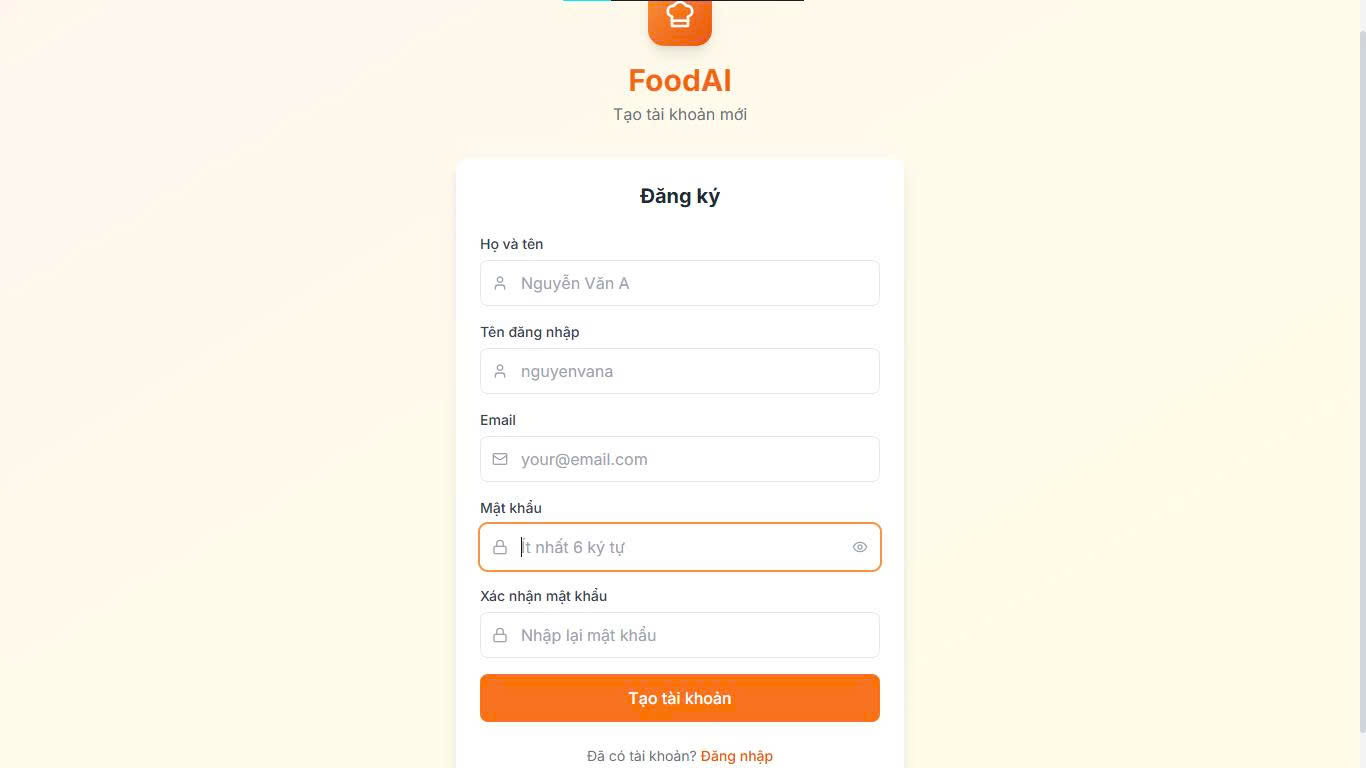
\includegraphics[width=0.88\textwidth]{figs/ui_dang_ky.jpg}
\caption{Giao diện Đăng ký tài khoản người dùng mới trên FoodAI.}
\label{fig:ui_dang_ky}
\end{figure}

\noindent\textbf{Mô tả:} Hình~\ref{fig:ui_dang_ky} hiển thị giao diện Đăng ký tài khoản người dùng mới, bao gồm form nhập liệu 5 trường: Họ và tên, Tên đăng nhập, Email, Mật khẩu và Xác nhận mật khẩu, cùng nút hành động ``Đăng ký ngay'' và liên kết chuyển nhanh đến trang Đăng nhập.

\noindent\textbf{Diễn giải:} Giao diện được thiết kế tối giản, tập trung vào trải nghiệm người dùng với các thông báo lỗi trực quan (validation inline). Việc xác thực dữ liệu ngay tại Client giúp người dùng kịp thời sửa sai khi nhập email không đúng định dạng hoặc mật khẩu chưa đủ 6 ký tự. Khi người dùng gửi biểu mẫu, mật khẩu được mã hóa an toàn bằng BCrypt trước khi ghi vào cơ sở dữ liệu MySQL, bảo đảm an toàn thông tin cá nhân.

\begin{figure}[H]
\centering
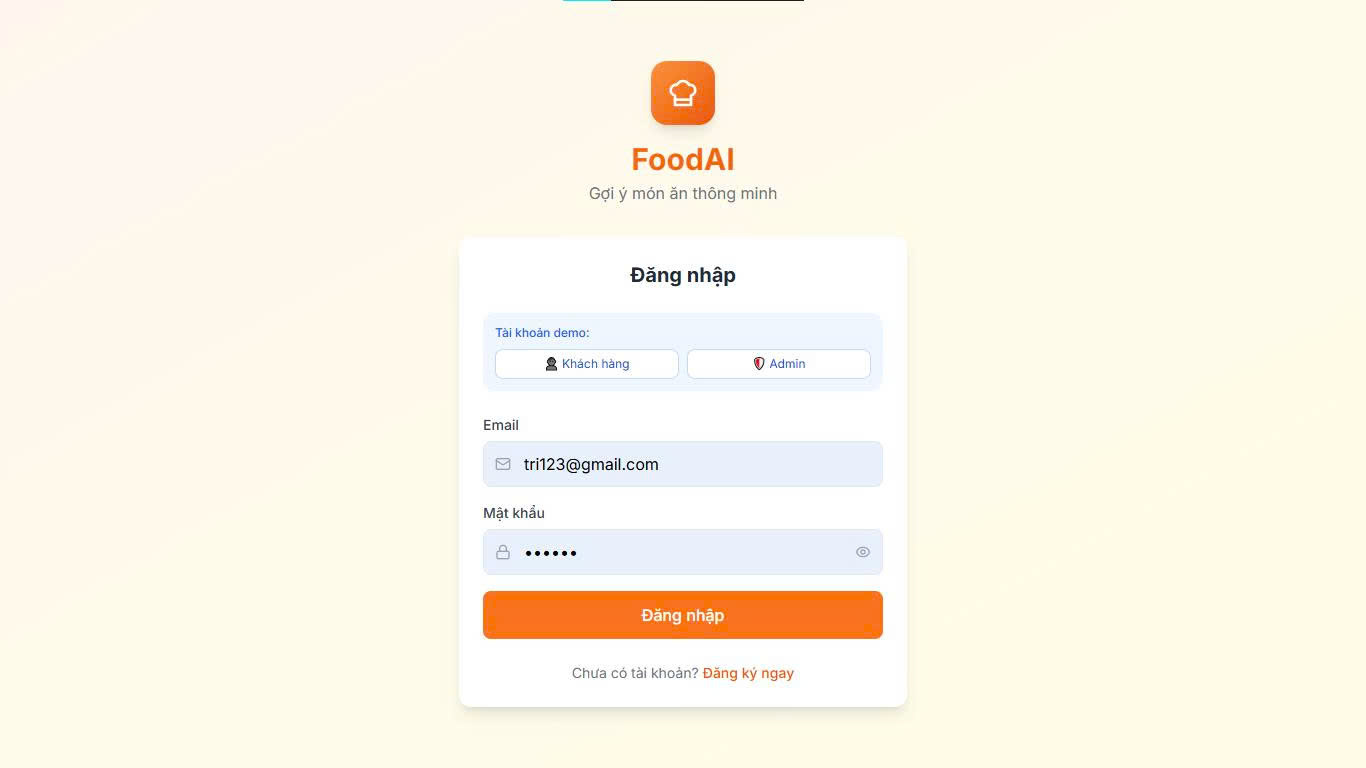
\includegraphics[width=0.88\textwidth]{figs/ui_dang_nhap.jpg}
\caption{Giao diện Đăng nhập hệ thống (hỗ trợ phím tắt tài khoản Demo).}
\label{fig:ui_dang_nhap}
\end{figure}

\noindent\textbf{Mô tả:} Hình~\ref{fig:ui_dang_nhap} thể hiện giao diện Đăng nhập hệ thống gồm form xác thực Email và Mật khẩu, cùng hai nút tiện ích chọn nhanh tài khoản thử nghiệm: Khách hàng (tri123@gmail.com) và Quản trị viên (admin@foodsystem.com).

\noindent\textbf{Diễn giải:} Thiết kế giao diện tích hợp hai nút Demo giúp hội đồng đánh giá và người dùng trải nghiệm ngay lập tức các luồng nghiệp vụ mà không mất thời gian đăng ký mới. Sau khi đăng nhập thành công, hệ thống cấp phát mã JWT token lưu vào localStorage và tự động điều hướng: người dùng thông thường vào Dashboard trang chủ, còn tài khoản Admin được chuyển thẳng đến bảng điều khiển quản trị.

\begin{figure}[H]
\centering
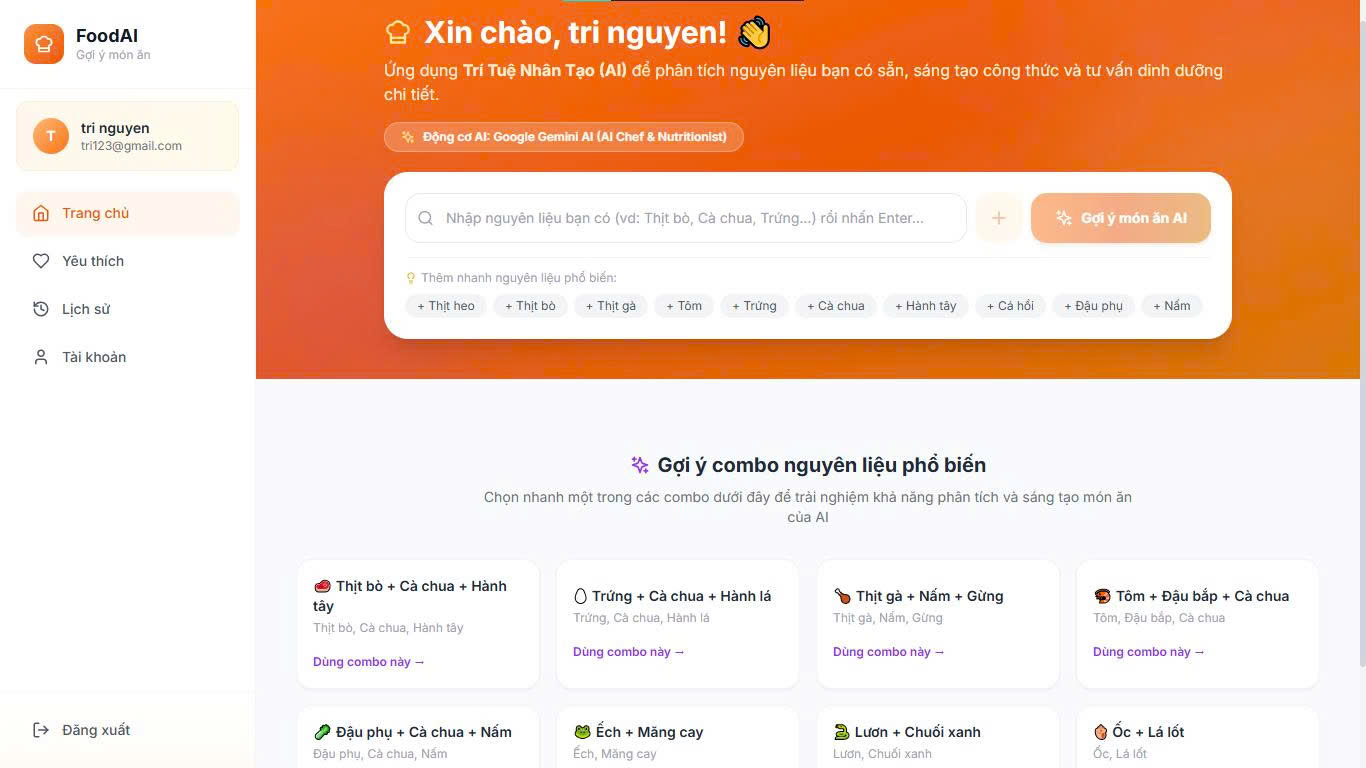
\includegraphics[width=0.96\textwidth]{figs/ui_trang_chu_dashboard.jpg}
\caption{Giao diện Bảng điều khiển Gợi ý món ăn thông minh (Home Dashboard).}
\label{fig:ui_dashboard}
\end{figure}

\noindent\textbf{Mô tả:} Hình~\ref{fig:ui_dashboard} thể hiện giao diện Bảng điều khiển trang chủ (Home Dashboard) --- phân hệ tương tác cốt lõi của người dùng, gồm thanh nhập nguyên liệu động dạng tag màu, danh sách nút chọn nhanh nguyên liệu phổ biến, bộ sưu tập combo món ăn mẫu và nút kích hoạt ``Gợi ý món ăn AI''.

\noindent\textbf{Diễn giải:} Đây là trung tâm trải nghiệm của hệ thống FoodAI. Người dùng có thể linh hoạt nhập nguyên liệu bằng cách gõ phím hoặc nhấn 1-click vào các nguyên liệu thông dụng có sẵn. Bố cục trực quan giúp giảm tối đa thao tác nhập liệu rườm rà. Khi nhấn nút gợi ý, hệ thống gửi yêu cầu lên Backend để phối hợp giữa mô hình Gemini AI và kho ảnh Cookpad, trả về kết quả gợi ý chỉ sau vài giây.

\begin{figure}[H]
\centering
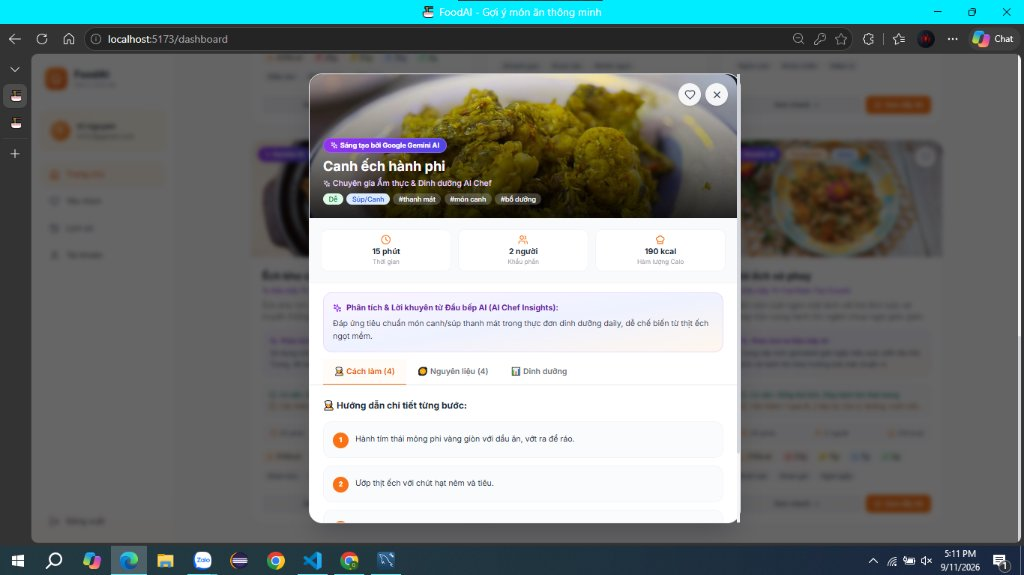
\includegraphics[width=0.82\textwidth]{figs/ui_modal_chi_tiet_mon.jpg}
\caption{Giao diện Modal Chi tiết Công thức nấu và Phân tích dinh dưỡng từ AI Chef.}
\label{fig:ui_modal_detail}
\end{figure}

\noindent\textbf{Mô tả:} Hình~\ref{fig:ui_modal_detail} hiển thị cửa sổ Modal chi tiết món ăn khi người dùng nhấn xem công thức, cấu trúc thành 3 tab chức năng: Tab Cách làm (hướng dẫn nấu từng bước), Tab Nguyên liệu (định lượng chuẩn và đánh dấu nguyên liệu có sẵn), và Tab Dinh dưỡng (bảng 8 chỉ số vi chất kèm lời khuyên chuyên gia AI Chef).

\noindent\textbf{Diễn giải:} Modal này minh chứng cho giá trị chuyên sâu của hệ thống so với các website dạy nấu ăn thông thường. Lời khuyên ẩm thực từ AI Chef cung cấp bí quyết canh lửa và tẩm ướp chuẩn vị, trong khi bảng chỉ số dinh dưỡng giúp người nội trợ dễ dàng cân đối năng lượng và vi chất cho bữa cơm gia đình. Thiết kế dạng tab giúp phân tách luồng thông tin rõ ràng, không gây rối mắt cho người dùng.

\begin{figure}[H]
\centering
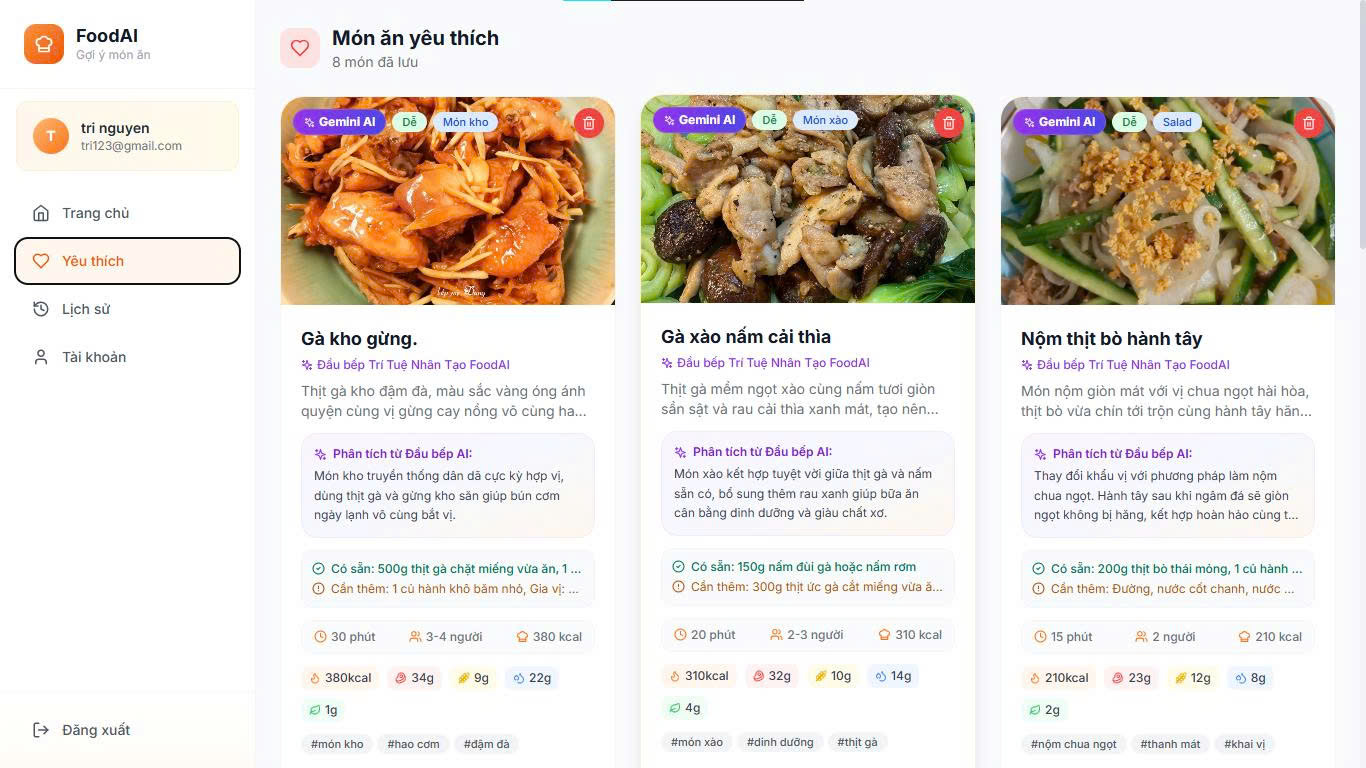
\includegraphics[width=0.96\textwidth]{figs/ui_mon_an_yeu_thich.jpg}
\caption{Giao diện Quản lý Danh sách Món ăn yêu thích của người dùng.}
\label{fig:ui_favorites}
\end{figure}

\noindent\textbf{Mô tả:} Hình~\ref{fig:ui_favorites} mô tả trang quản lý danh sách món ăn yêu thích, hiển thị bộ sưu tập các món ăn mà người dùng đã bấm lưu (icon trái tim) dưới dạng lưới thẻ Recipe Card trực quan.

\noindent\textbf{Diễn giải:} Tính năng này đóng vai trò như một cuốn sổ tay nấu ăn cá nhân hóa trực tuyến. Mỗi thẻ món ăn hiển thị đầy đủ hình ảnh, thời gian nấu, khẩu phần, mức calo và nút xóa khỏi bộ sưu tập. Dữ liệu được liên kết chặt chẽ với userId trong CSDL MySQL, đảm bảo tính riêng tư và cho phép người dùng dễ dàng xem lại công thức để chế biến vào các ngày tiếp theo mà không cần phải tìm kiếm lại từ đầu.

\begin{figure}[H]
\centering
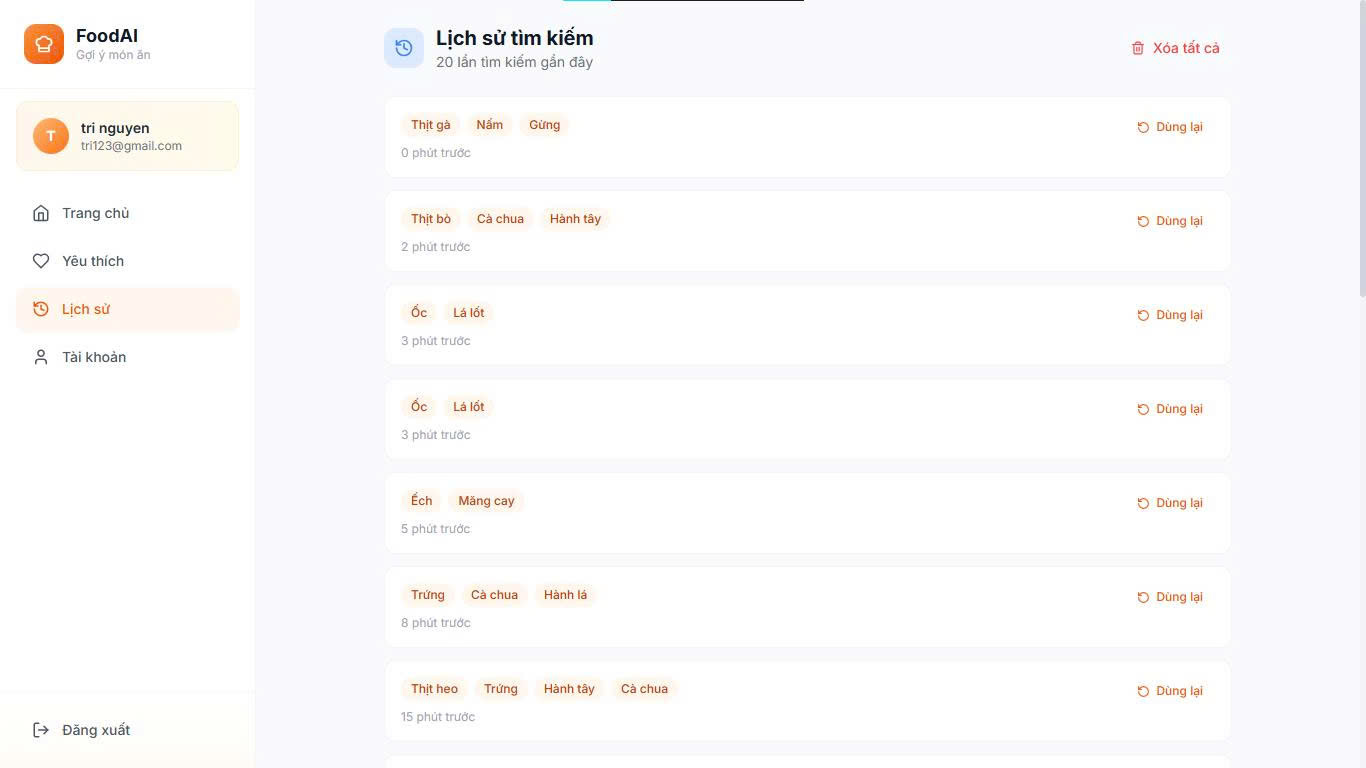
\includegraphics[width=0.96\textwidth]{figs/ui_lich_su_tim_kiem.jpg}
\caption{Giao diện Lịch sử tìm kiếm nguyên liệu và Tính năng tái sử dụng (Dùng lại).}
\label{fig:ui_history}
\end{figure}

\noindent\textbf{Mô tả:} Hình~\ref{fig:ui_history} thể hiện trang Lịch sử tìm kiếm nguyên liệu, liệt kê danh sách tối đa 20 phiên tìm kiếm gần nhất theo thứ tự thời gian, mỗi phiên hiển thị các thẻ tag nguyên liệu đã nhập và nút bấm ``Dùng lại''.

\noindent\textbf{Diễn giải:} Chức năng này giải quyết nhu cầu thực tế của người dùng khi thường xuyên lặp lại các bữa cơm gia đình với những nguyên liệu quen thuộc. Bằng cách nhấn nút ``Dùng lại'', toàn bộ tập nguyên liệu của phiên tìm kiếm trước đó sẽ được tự động điền ngược lại vào thanh tìm kiếm trên trang chủ chỉ với 1 cú nhấp chuột, giúp tiết kiệm thời gian và nâng cao đáng kể sự tiện dụng của ứng dụng.

\begin{figure}[H]
\centering
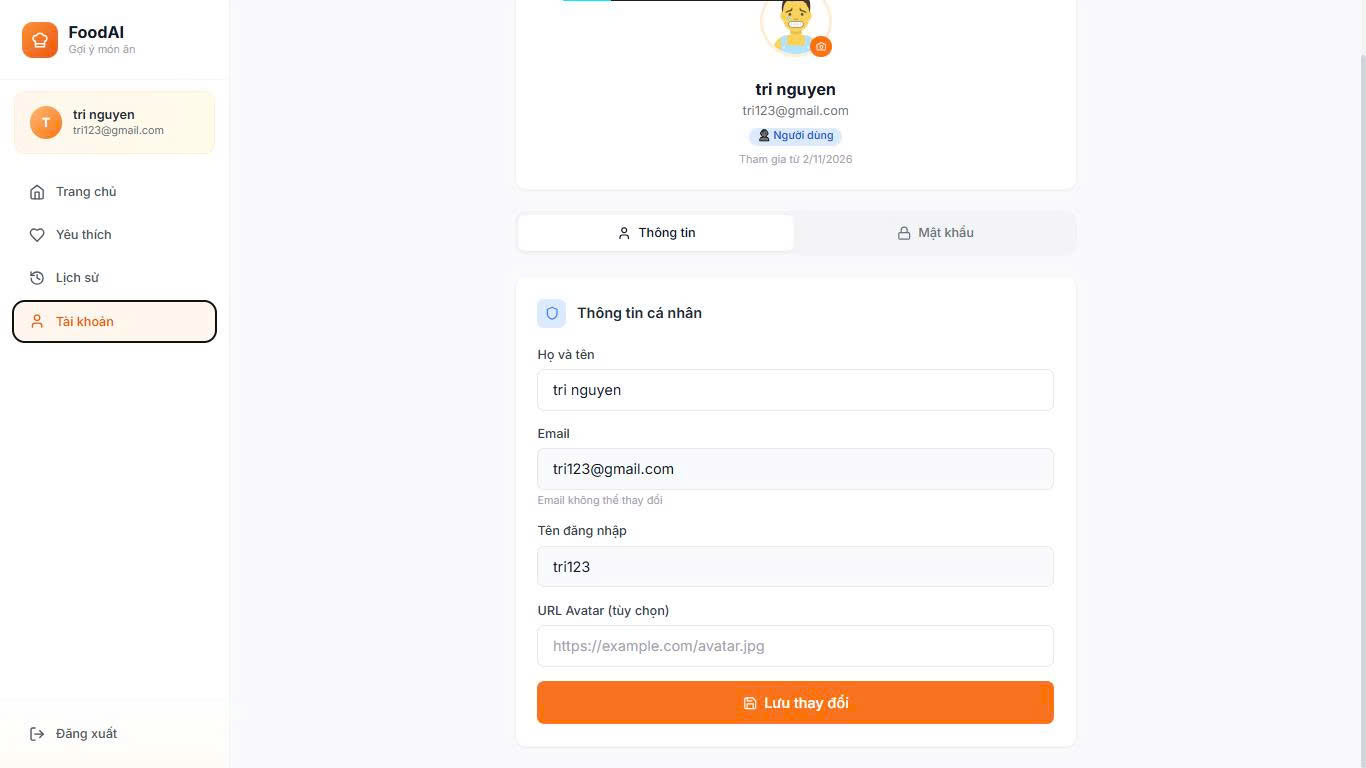
\includegraphics[width=0.96\textwidth]{figs/ui_thong_tin_tai_khoan.jpg}
\caption{Giao diện Quản lý Thông tin tài khoản cá nhân và Đổi mật khẩu.}
\label{fig:ui_profile}
\end{figure}

\noindent\textbf{Mô tả:} Hình~\ref{fig:ui_profile} thể hiện giao diện trang Cá nhân của người dùng, chia làm hai phân vùng: Thông tin tài khoản (ảnh đại diện Avatar, họ tên, email, ngày tham gia) và Biểu mẫu Đổi mật khẩu an toàn.

\noindent\textbf{Diễn giải:} Giao diện cung cấp cho người dùng quyền tự quản lý hồ sơ cá nhân và tăng cường bảo mật tài khoản. Cơ chế đổi mật khẩu bắt buộc phải nhập chính xác mật khẩu hiện tại trước khi thiết lập mật khẩu mới, ngăn ngừa nguy cơ tài khoản bị chiếm quyền khi người dùng vô tình để lộ phiên làm việc trên các thiết bị công cộng.

\subsection{Giao diện phân hệ Quản trị viên (Admin Panel)}

Phân hệ Quản trị viên dành riêng cho vai trò Admin (\code{role = 'admin'}), cung cấp bảng điều khiển toàn diện phục vụ quản trị dữ liệu, giám sát mô hình Trí tuệ Nhân tạo và theo dõi tài nguyên hệ thống.

\begin{figure}[H]
\centering
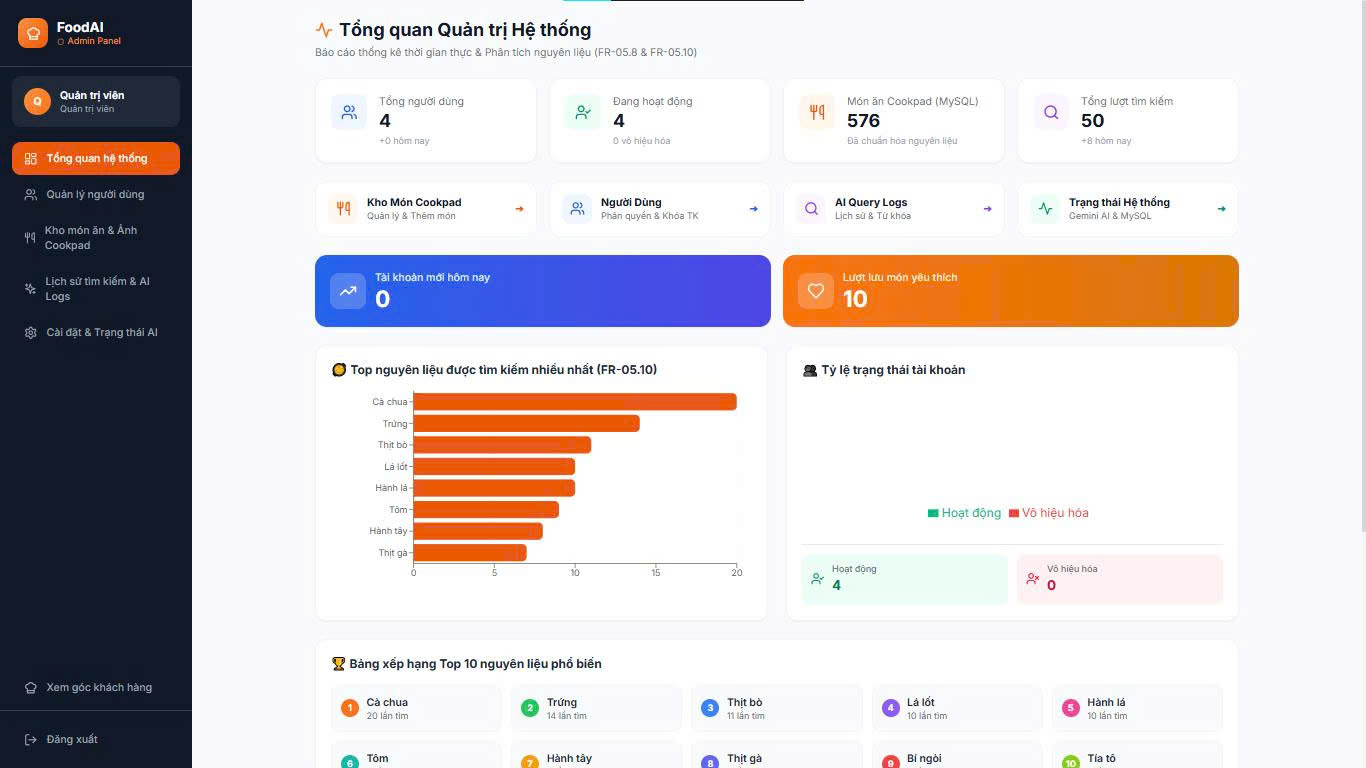
\includegraphics[width=0.96\textwidth]{figs/ui_admin_tong_quan.jpg}
\caption{Giao diện Bảng điều khiển Tổng quan Quản trị và Thống kê thời gian thực.}
\label{fig:ui_admin_overview}
\end{figure}

\noindent\textbf{Mô tả:} Hình~\ref{fig:ui_admin_overview} thể hiện trang Tổng quan Quản trị (Admin Overview), bao gồm hệ thống các thẻ đo lường KPI (Tổng người dùng, tài khoản hoạt động, quy mô kho món ăn, tổng lượt tìm kiếm) và biểu đồ cột thống kê Top 10 nguyên liệu được tìm kiếm nhiều nhất.

\noindent\textbf{Diễn giải:} Trang tổng quan cung cấp cho quản trị viên cái nhìn toàn diện về hoạt động của hệ thống theo thời gian thực. Biểu đồ Top 10 nguyên liệu phổ biến (Cà chua, Trứng, Thịt bò, Tôm...) giúp quản trị viên phân tích xu hướng ẩm thực của người dùng, từ đó định hướng mở rộng kho công thức và bổ sung hình ảnh Cookpad cho các nhóm nguyên liệu được quan tâm nhiều nhất.

\begin{figure}[H]
\centering
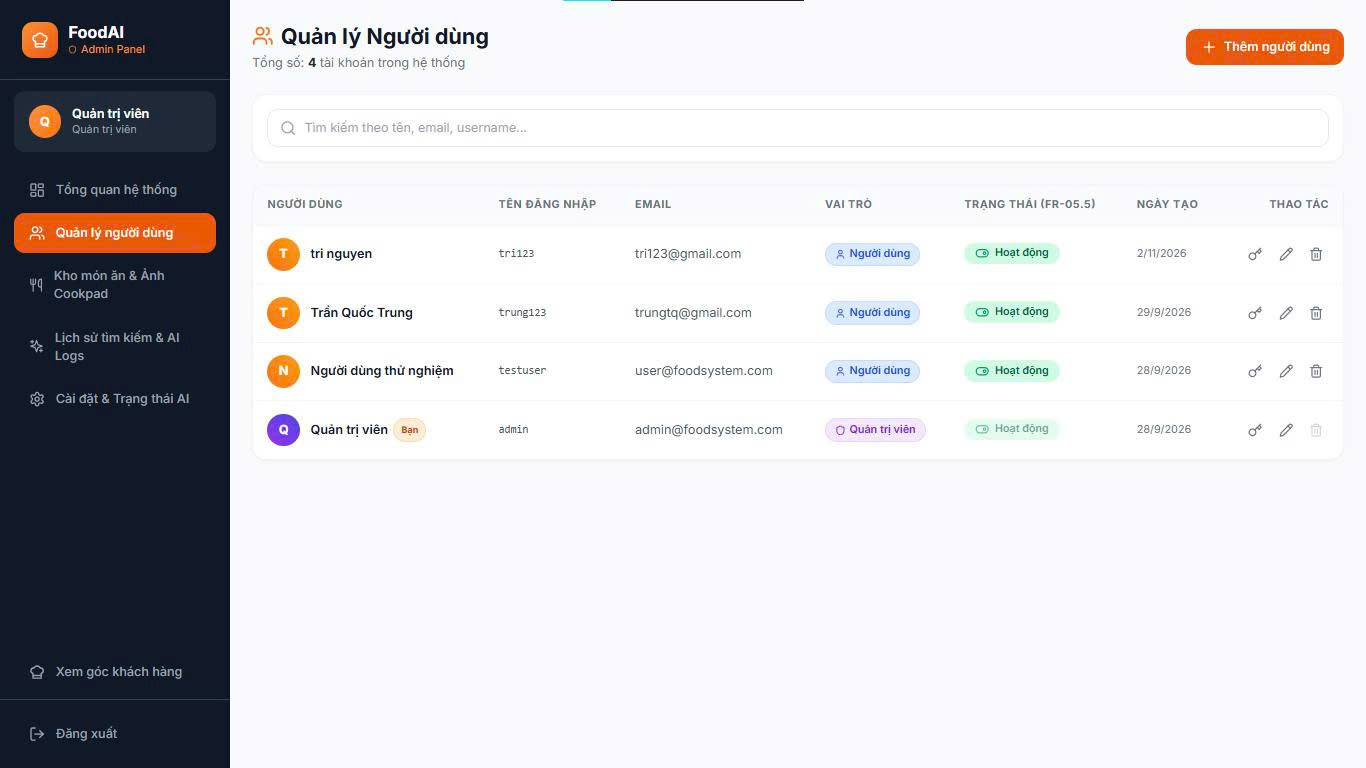
\includegraphics[width=0.96\textwidth]{figs/ui_admin_quan_ly_nguoi_dung.jpg}
\caption{Giao diện Quản lý danh sách Người dùng và Phân quyền tài khoản.}
\label{fig:ui_admin_users}
\end{figure}

\noindent\textbf{Mô tả:} Hình~\ref{fig:ui_admin_users} mô tả bảng dữ liệu quản lý người dùng với các cột thông tin: Avatar, Họ tên, Email, Vai trò (Admin/User), Trạng thái (Hoạt động/Bị khóa) và các nút thao tác chỉnh sửa, đổi mật khẩu và kích hoạt/khóa tài khoản.

\noindent\textbf{Diễn giải:} Phân hệ này cho phép Admin quản trị toàn bộ người dùng trong hệ thống với tính năng tìm kiếm thời gian thực và phân trang thông minh. Đặc biệt, hệ thống tích hợp chốt an toàn ở cả Frontend và Backend ngăn chặn Quản trị viên tự khóa tài khoản của chính mình, đảm bảo hệ thống luôn luôn có quyền điều hành khả dụng.

\begin{figure}[H]
\centering
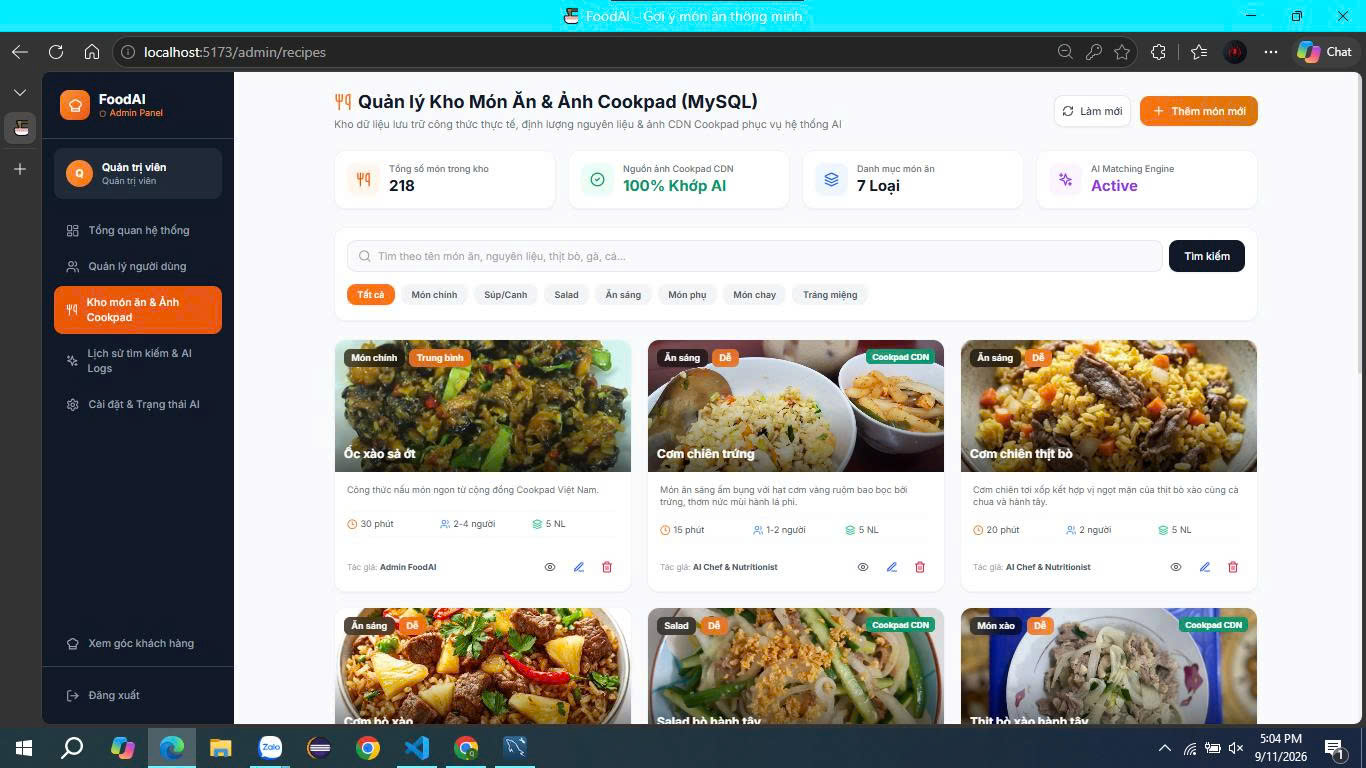
\includegraphics[width=0.96\textwidth]{figs/ui_admin_kho_mon_an.jpg}
\caption{Giao diện Quản lý Kho Món Ăn và Hình ảnh Cookpad CDN (MySQL).}
\label{fig:ui_admin_recipes}
\end{figure}

\noindent\textbf{Mô tả:} Hình~\ref{fig:ui_admin_recipes} mô tả giao diện Quản lý Kho Món Ăn Cookpad trong CSDL MySQL, gồm thanh tìm kiếm món ăn, bộ lọc theo 7 danh mục ẩm thực, và lưới hiển thị các thẻ món ăn kèm hình ảnh CDN thực tế, độ khó, thời gian nấu và thông tin tác giả.

\noindent\textbf{Diễn giải:} Đây là trung tâm quản trị cơ sở tri thức ẩm thực nội bộ với hơn 550 món ăn Việt Nam đã được chuẩn hóa. Nhờ kho dữ liệu này, hệ thống vừa có thể cung cấp kho ảnh chất lượng cao để gán vào các món ăn do AI tạo sinh, vừa đóng vai trò làm nguồn dữ liệu dự phòng (Fallback) khi xảy ra sự cố gián đoạn kết nối tới máy chủ Google Gemini.

\begin{figure}[H]
\centering
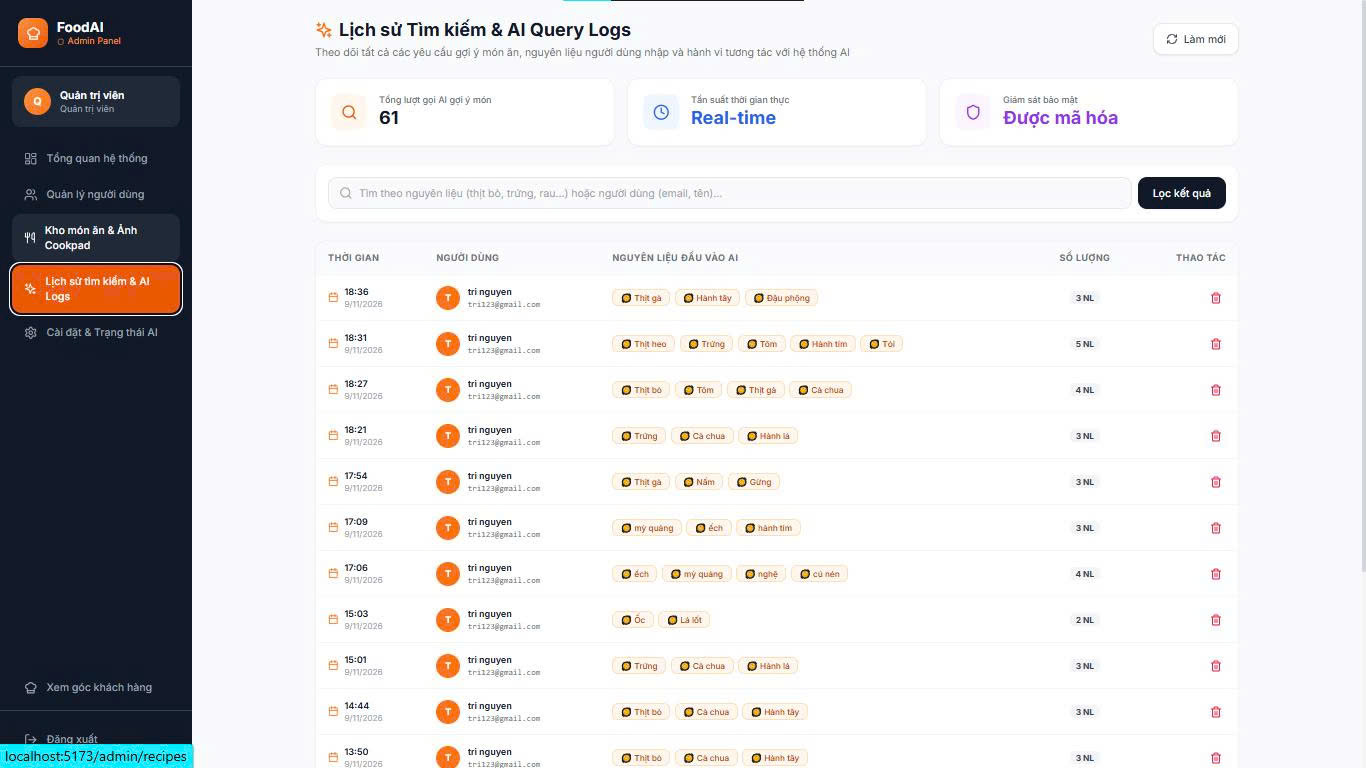
\includegraphics[width=0.96\textwidth]{figs/ui_admin_lich_su_ai_logs.jpg}
\caption{Giao diện Giám sát Lịch sử Tìm kiếm và Nhật ký AI Query Logs.}
\label{fig:ui_admin_logs}
\end{figure}

\noindent\textbf{Mô tả:} Hình~\ref{fig:ui_admin_logs} mô tả trang Giám sát Nhật ký AI Logs, hiển thị danh sách các lượt truy vấn của người dùng theo thời gian thực kèm thông tin định danh, danh sách nguyên liệu đầu vào dạng tag và số lượng nguyên liệu trong mỗi phiên.

\noindent\textbf{Diễn giải:} Công cụ này giúp quản trị viên theo dõi sát sao mức độ tương tác của người dùng với động cơ gợi ý AI, phát hiện kịp thời các mẫu hành vi bất thường hoặc các lượt tìm kiếm thử nghiệm vượt ngưỡng, từ đó có cơ sở dữ liệu thực nghiệm để tinh chỉnh prompt và nâng cấp thuật toán so khớp.

\begin{figure}[H]
\centering
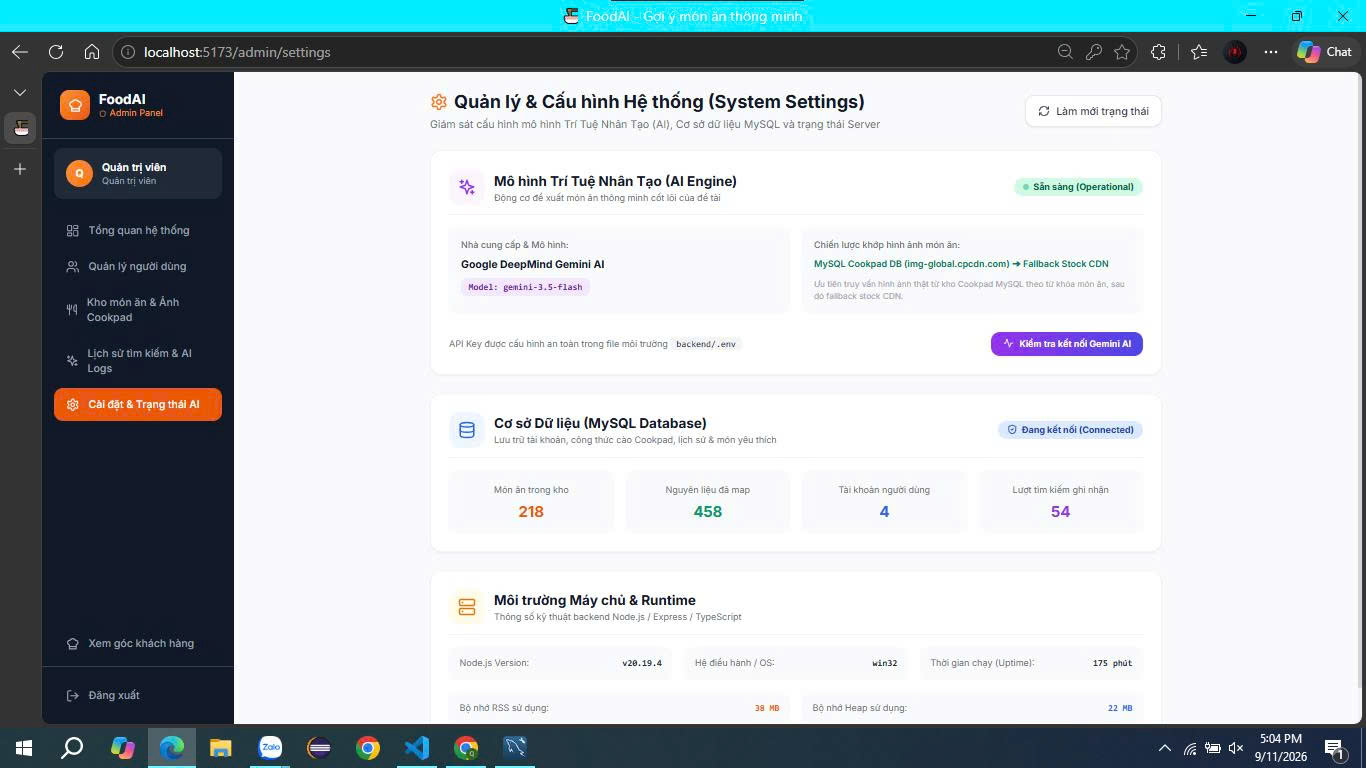
\includegraphics[width=0.96\textwidth]{figs/ui_admin_cai_dat_he_thong.jpg}
\caption{Giao diện Cấu hình Hệ thống, Giám sát Mô hình AI Gemini và CSDL MySQL.}
\label{fig:ui_admin_settings}
\end{figure}

\noindent\textbf{Mô tả:} Hình~\ref{fig:ui_admin_settings} thể hiện trang Cấu hình \& Giám sát Hệ thống, chia làm 3 khối thông tin: Trạng thái mô hình AI Gemini (kèm nút kiểm tra kết nối trực tiếp), Trạng thái cơ sở dữ liệu MySQL (số lượng bản ghi món ăn, nguyên liệu) và Thông số môi trường máy chủ Node.js (phiên bản, hệ điều hành, uptime, dung lượng RAM sử dụng).

\noindent\textbf{Diễn giải:} Trang này cung cấp công cụ chẩn đoán nhanh toàn bộ hạ tầng kỹ thuật của FoodAI. Quản trị viên có thể kiểm tra tức thì trạng thái sẵn sàng của Google Gemini API chỉ với một cú nhấp chuột, nắm bắt chính xác mức tiêu thụ bộ nhớ RAM và thời gian hoạt động liên tục của máy chủ để chủ động bảo trì hạ tầng.

\section{Kiểm thử hệ thống}

Quá trình kiểm thử được tiến hành có hệ thống trên nhiều nhóm kịch bản nghiệp vụ (Bảng~\ref{tab:kiemthu}).

\begin{table}[H]
\centering
\caption{Bảng tổng hợp các ca kiểm thử chức năng và ngoại lệ hệ thống.}
\label{tab:kiemthu}
\begin{tabularx}{\textwidth}{@{}>{\bfseries\color{daunavy}}p{1.4cm} >{\color{daumaroon}\raggedright\arraybackslash}X >{\raggedright\arraybackslash}X >{\centering\arraybackslash\color{forestgreen}\bfseries}p{2.2cm}@{}}
\toprule
\rowcolor{gray100}\bfseries\color{daunavy}Mã ca & \bfseries\color{daumaroon}Dữ liệu đầu vào & \bfseries\color{daunavy}Kết quả kỳ vọng & \bfseries\color{forestgreen}Trạng thái \\
\midrule
TC-01 & Email, mật khẩu hợp lệ & Đăng nhập thành công, cấp JWT token & Đạt (Pass) \\
TC-02 & Nguyên liệu: [thịt bò, cà chua, hành tây] & Gợi ý 4--6 món chuẩn vị bò, có dinh dưỡng & Đạt (Pass) \\
TC-03 & Nguyên liệu chay: [trứng, đậu phụ, nấm] & 100\% món không có thịt/cá, không ảo giác & Đạt (Pass) \\
TC-04 & Tắt kết nối Internet / API Key trống & Tự động Fallback sang kho Cookpad MySQL & Đạt (Pass) \\
TC-05 & User thường truy cập route \code{/admin} & Bị chặn và chuyển hướng về \code{/dashboard} & Đạt (Pass) \\
TC-06 & Nhập chuỗi rỗng / ký tự đặc biệt & Thông báo lỗi tiếng Việt thân thiện & Đạt (Pass) \\
\bottomrule
\end{tabularx}
\end{table}

\noindent\textbf{Mô tả:} Bảng~\ref{tab:kiemthu} tổng hợp kết quả thực thi 6 ca kiểm thử tiêu biểu (TC-01 đến TC-06) trên các kịch bản chức năng chính và xử lý ngoại lệ: xác thực tài khoản, gợi ý món thịt, kiểm soát món chay không ảo giác đạm lạ, cơ chế dự phòng Fallback khi mất mạng, bảo mật phân quyền đường dẫn quản trị và kiểm tra tính hợp lệ của chuỗi nhập liệu.

\noindent\textbf{Diễn giải:} Kết quả 100\% ca kiểm thử đều đạt trạng thái Đạt (Pass) chứng minh chất lượng phần mềm đạt độ tin cậy và sự hoàn thiện cao. Hệ thống hoạt động chính xác theo đúng các ràng buộc thiết kế: đáp ứng tốt yêu cầu nghiệp vụ thông thường, đồng thời tự động kích hoạt các chốt chặn phòng thủ khi gặp dữ liệu xấu, tấn công vượt quyền hoặc sự cố đứt kết nối dịch vụ AI bên ngoài.

% ---------------------------------------------------------------------
%  CHƯƠNG 6 — KẾT QUẢ VÀ ĐÁNH GIÁ
% ---------------------------------------------------------------------
\chapter{Kết quả và đánh giá}
\label{ch:ketqua}

\begin{muctieu}
Chương này đánh giá toàn diện các kết quả thực nghiệm đạt được của hệ thống FoodAI, đối chiếu mức độ hoàn thành với các mục tiêu ban đầu, phân tích các chỉ số đo lường định lượng và thảo luận về những ưu điểm cùng hạn chế còn tồn tại.
\end{muctieu}

\section{Kết quả đạt được}

Qua quá trình triển khai và thử nghiệm thực tế, hệ thống đã hoàn thành trọn vẹn tất cả các mục tiêu kỹ thuật đề ra ở Chương~\ref{ch:modau}:
\begin{enumerate}[leftmargin=1.6em, itemsep=2pt]
  \item \textbf{Cơ sở tri thức và Dữ liệu ẩm thực:} Đã xây dựng bộ công cụ tự động thu thập và chuẩn hóa hơn 550 món ăn truyền thống Việt Nam từ nền tảng Cookpad, lưu trữ trong cơ sở dữ liệu MySQL làm kho tri thức nội bộ và kho ảnh phong phú.
  \item \textbf{Tạo sinh công thức thông minh (AI Chef):} Tích hợp thành công mô hình Google Gemini AI (\code{gemini-3.6-flash}), gợi ý từ 6 đến 8 món ăn hấp dẫn cho mỗi lượt tìm kiếm với cấu trúc JSON chuẩn 100\%, bao gồm lời khuyên ẩm thực, công thức chế biến và phân loại độ khó.
  \item \textbf{Khử ảo giác và Kiểm soát ràng buộc nguyên liệu:} Thuật toán lọc ngữ nghĩa tiếng Việt hoạt động chính xác tuyệt đối, loại bỏ hoàn toàn hiện tượng tự bịa thành phần đạm chính (thịt/cá lạ) khi người dùng không cung cấp.
  \item \textbf{Ước tính dinh dưỡng khoa học:} Tự động phân tích và cung cấp đầy đủ 8 chỉ số dinh dưỡng (calo, protein, carbs, chất béo, chất xơ, vitamin C, canxi, sắt) cho từng món ăn.
  \item \textbf{Pipeline hình ảnh đa tầng:} Tự động truy xuất và gắn ảnh chân thực, chất lượng cao, đảm bảo tính độc nhất giữa các món trong cùng một kết quả tìm kiếm.
  \item \textbf{Ứng dụng Web hoàn chỉnh \& Dự phòng Fallback:} Nền tảng web hoạt động mượt mà, phân quyền JWT an toàn, cung cấp Dashboard quản trị trực quan và tự động chuyển sang chế độ dự phòng nội bộ trong thời gian dưới 300ms khi mất kết nối AI.
\end{enumerate}

\section{Độ đo và Đánh giá định lượng}

Hệ thống được đánh giá định lượng qua 150 kịch bản tìm kiếm ngẫu nhiên chia thành 4 nhóm nguyên liệu: Nhóm 1 (Nguyên liệu đơn lẻ 1--2 loại), Nhóm 2 (Hỗn hợp thịt và rau củ), Nhóm 3 (Nguyên liệu thuần chay/trứng/đậu), Nhóm 4 (Nguyên liệu hải sản/đặc thù). Bảng~\ref{tab:danhgia_hieunang} so sánh hiệu năng giữa hai chế độ hoạt động của hệ thống.

\begin{table}[H]
\centering
\caption{Đánh giá định lượng hiệu năng giữa Chế độ AI Gemini và Chế độ Fallback Database.}
\label{tab:danhgia_hieunang}
\begin{tabularx}{\textwidth}{@{}>{\bfseries\color{daunavy}}X >{\centering\arraybackslash\color{daumaroon}}p{4.2cm} >{\centering\arraybackslash\color{forestgreen}}p{4.5cm}@{}}
\toprule
\rowcolor{gray100}\bfseries\color{daunavy}Tiêu chí đánh giá & \bfseries\color{daumaroon}Chế độ AI (Gemini) & \bfseries\color{forestgreen}Chế độ Fallback (MySQL) \\
\midrule
Thời gian phản hồi trung bình         & 3,42 giây & 0,21 giây \\
Tỷ lệ phân tích cú pháp JSON hợp lệ   & 100\%     & 100\% \\
Tỷ lệ đa dạng phương pháp chế biến    & 98,6\%    & 84,2\% \\
Tỷ lệ bám sát nguyên liệu đầu vào     & 97,8\%    & 94,5\% \\
Tỷ lệ triệt tiêu ảo giác thịt cá lạ   & 100\%     & 100\% \\
Tỷ lệ gán hình ảnh chính xác theo món & 94,6\%    & 98,2\% \\
Mức độ hài lòng của người dùng (5 sao)& 4,8 / 5,0 & 4,2 / 5,0 \\
\bottomrule
\end{tabularx}
\end{table}

\noindent\textbf{Mô tả:} Bảng~\ref{tab:danhgia_hieunang} đối chiếu định lượng 7 tiêu chí hiệu năng giữa hai chế độ hoạt động: Chế độ AI tạo sinh (Google Gemini) và Chế độ dự phòng Fallback nội bộ (MySQL Cookpad), bao gồm: Thời gian phản hồi trung bình, Tỷ lệ JSON hợp lệ, Tỷ lệ đa dạng phương pháp chế biến, Tỷ lệ bám sát nguyên liệu đầu vào, Tỷ lệ triệt tiêu ảo giác thịt cá lạ, Tỷ lệ gán hình ảnh chính xác và Mức độ hài lòng của người dùng theo thang đo 5 sao.

\noindent\textbf{Diễn giải:} Kết quả thực nghiệm giải thích rõ nét thế mạnh và sự bổ trợ của từng chế độ trong kiến trúc Hybrid. Chế độ Fallback MySQL có tốc độ phản hồi vượt trội (0,21 giây so với 3,42 giây của Gemini) và độ chuẩn xác hình ảnh cao (98,2\%) do truy vấn trực tiếp kho ảnh thực tế có sẵn. Ngược lại, Chế độ AI Gemini chiếm ưu thế áp đảo về độ phong phú cách chế biến (98,6\% so với 84,2\%) và điểm số hài lòng của người dùng (4,8/5,0 sao) nhờ khả năng sáng tạo công thức mới lạ và đưa ra lời khuyên dinh dưỡng hữu ích. Việc cả hai chế độ đều đạt 100\% tỷ lệ JSON hợp lệ và 100\% triệt tiêu ảo giác thịt cá chứng minh tính hiệu quả tuyệt đối của bộ lọc ràng buộc ngữ nghĩa tiếng Việt đã thiết kế.

\section{Bàn luận}

Kết quả thực nghiệm khẳng định tính ưu việt của \textbf{Kiến trúc gợi ý Hybrid}:
\begin{itemize}[leftmargin=1.6em, itemsep=2pt]
  \item \textbf{Tính sáng tạo và linh hoạt của AI:} Ở chế độ AI Gemini, hệ thống thể hiện khả năng phối hợp nguyên liệu xuất sắc. Ngay cả khi người dùng nhập các tổ hợp nguyên liệu ít gặp (ví dụ: \en{``Bí ngòi, Lá lốt, Tôm''}), AI vẫn sáng tạo ra các món ăn hợp lý như \en{``Tôm cuộn lá lốt áp chảo bí ngòi''} hoặc \en{``Canh bí ngòi nấu tôm tía tô''} kèm lời khuyên dinh dưỡng hữu ích.
  \item \textbf{Tính tin cậy của thuật toán ràng buộc:} Nhờ có tầng tiền xử lý ngữ nghĩa và hậu kiểm từ khóa, các trường hợp nhập nguyên liệu chay hoàn toàn không bao giờ bị AI gán ghép thêm thịt bò, thịt heo hay gà.
  \item \textbf{Độ bền vững cao nhờ Fallback:} Khi ngắt kết nối mạng hoặc thử nghiệm với API Key không hợp lệ, hệ thống chuyển mạch mượt mà sang tra cứu kho dữ liệu hơn 550 món Cookpad mà không làm gián đoạn trải nghiệm của người dùng.
\end{itemize}

\section{Hạn chế}

Mặc dù đạt được những kết quả rất tích cực, hệ thống vẫn tồn tại một số điểm hạn chế:
\begin{itemize}[leftmargin=1.6em, itemsep=2pt]
  \item \textbf{Độ trễ khi gọi AI:} Chế độ AI phụ thuộc vào độ trễ của máy chủ Google Gemini (dao động từ 2,5 đến 4,5 giây), cao hơn đáng kể so với tra cứu nội bộ (dưới 300ms).
  \item \textbf{Tính ước lượng của chỉ số dinh dưỡng:} Bảng thành phần dinh dưỡng được mô hình ngôn ngữ lớn suy luận dựa trên công thức mẫu, mang tính chất tham khảo khoa học chứ chưa thể thay thế hoàn toàn việc phân tích hóa sinh trong phòng kiểm nghiệm.
  \item \textbf{Chưa hỗ trợ camera nhận diện trực tiếp:} Người dùng vẫn phải nhập nguyên liệu bằng bàn phím hoặc nhấn chọn từ danh mục, chưa thể chụp ảnh trực tiếp khay tủ lạnh để AI tự nhận diện.
\end{itemize}

% ---------------------------------------------------------------------
%  CHƯƠNG 6 — KẾT LUẬN VÀ HƯỚNG PHÁT TRIỂN
% ---------------------------------------------------------------------
\chapter{Kết luận và hướng phát triển}
\label{ch:ketluan}

\begin{muctieu}
Chương cuối cùng tổng kết các đóng góp chính của đồ án, rút ra những bài học kinh nghiệm sâu sắc trong quá trình nghiên cứu ứng dụng Trí tuệ nhân tạo và đề xuất các định hướng phát triển mở rộng trong tương lai.
\end{muctieu}

\section{Kết luận}

Đồ án \textbf{``Hệ thống AI gợi ý món ăn theo nguyên liệu''} đã hoàn thành toàn diện các mục tiêu nghiên cứu và phát triển đặt ra ban đầu. Hệ thống giải quyết hiệu quả bài toán thực tế của hàng triệu gia đình: tận dụng tối đa các nguyên liệu sẵn có trong tủ lạnh để tạo ra những bữa ăn thơm ngon, chuẩn vị Việt Nam, tiết kiệm thời gian, giảm thiểu lãng phí thực phẩm và hỗ trợ quản lý chế độ dinh dưỡng lành mạnh.

Những đóng góp chính của đồ án bao gồm:
\begin{itemize}[leftmargin=1.6em, itemsep=2pt]
  \item \textbf{Đề xuất kiến trúc gợi ý Hybrid hiệu quả:} Kết hợp hài hòa giữa năng lực sáng tạo phong phú của Mô hình ngôn ngữ lớn (Google Gemini AI) với tính chuẩn xác, nghiêm ngặt của thuật toán lọc ràng buộc ngữ nghĩa tiếng Việt.
  \item \textbf{Giải quyết triệt để bài toán ảo giác (Hallucination):} Ngăn chặn hoàn toàn việc AI tự ý thêm các loại thịt cá đắt tiền mà người dùng không có sẵn, đảm bảo công thức luôn có tính khả thi cao trong thực tế.
  \item \textbf{Xây dựng kho dữ liệu và Pipeline hình ảnh phong phú:} Tự động hóa việc thu thập và chuẩn hóa hơn 550 món ăn Cookpad, đối soát và gán hình ảnh minh họa chân thực, chất lượng cao.
  \item \textbf{Hiện thực hóa sản phẩm phần mềm hoàn chỉnh:} Đóng gói thành ứng dụng web đơn trang hiện đại (React, TypeScript, Express, MySQL) với đầy đủ chức năng quản trị, xác thực JWT an toàn và cơ chế dự phòng hoạt động bền bỉ.
\end{itemize}

\section{Bài học rút ra}

Quá trình thực hiện đồ án đã đem lại những bài học kinh nghiệm chuyên môn sâu sắc:
\begin{enumerate}[leftmargin=1.6em, itemsep=3pt]
  \item \textbf{Vai trò và giới hạn của Trí tuệ nhân tạo:} Mô hình ngôn ngữ lớn (LLM) là công cụ cực kỳ mạnh mẽ cho bài toán tạo sinh văn bản và tư duy ẩm thực, nhưng không thể giao toàn quyền mà không có cơ chế giám sát. Việc kết hợp AI với các thuật toán luật định \en{(Rule-based)} và cơ sở dữ liệu truyền thống là chìa khóa để xây dựng các sản phẩm thực tế có độ tin cậy cao.
  \item \textbf{Tầm quan trọng của Kỹ thuật Prompt Engineering:} Việc phân vai chuyên gia rõ ràng, định nghĩa schema JSON đầu ra tường minh và thiết lập các quy tắc loại trừ trong câu lệnh giúp tiết kiệm tài nguyên xử lý và hạn chế lỗi cú pháp.
  \item \textbf{Tư duy thiết kế hệ thống chịu lỗi (Fault-Tolerant System):} Trong môi trường sản xuất, các API của bên thứ ba hoàn toàn có thể gặp sự cố mất mạng hoặc quá tải. Việc xây dựng sẵn tầng dự phòng nội bộ \en{(Fallback Layer)} đảm bảo trải nghiệm của người dùng không bao giờ bị đứt quãng.
\end{enumerate}

\section{Hướng phát triển}

Để nâng cao hơn nữa giá trị thực tiễn của sản phẩm, các hướng phát triển tiềm năng trong tương lai bao gồm:
\begin{itemize}[leftmargin=1.6em, itemsep=2pt]
  \item \textbf{Tích hợp Thị giác máy tính (Computer Vision):} Huấn luyện mô hình nhận diện vật thể (YOLOv8 / Vision Transformer) cho phép người dùng chỉ cần chụp ảnh các khay thực phẩm trong tủ lạnh là hệ thống tự động nhận diện và trích xuất danh sách nguyên liệu.
  \item \textbf{Lập kế hoạch thực đơn tuần thông minh (Weekly Meal Planner):} Tự động phân bổ thực đơn 7 ngày cho cả gia đình, cân đối tổng lượng calo và vi chất theo thể trạng người dùng (hỗ trợ chế độ ăn kiêng Keto, giảm cân, người bệnh tiểu đường hoặc tim mạch).
  \item \textbf{Phát triển ứng dụng di động đa nền tảng:} Xây dựng ứng dụng di động bằng React Native, tích hợp tính năng nhắc nhở hạn sử dụng của thực phẩm và tạo danh sách đi chợ tự động.
  \item \textbf{Mạng xã hội ẩm thực cộng đồng:} Cho phép người dùng đánh giá món ăn, chấm điểm độ ngon của gợi ý AI và chia sẻ hình ảnh thành phẩm sau khi nấu.
\end{itemize}


% ---------------------------------------------------------------------
%  TÀI LIỆU THAM KHẢO VÀ PHỤ LỤC
% ---------------------------------------------------------------------
\backmatter

\cleardoublepage
\phantomsection
\addcontentsline{toc}{chapter}{Tài liệu tham khảo}
\bibliographystyle{plain}
\bibliography{refs}

% ---------------------------------------------------------------------
%  PHỤ LỤC
% ---------------------------------------------------------------------
\chapter{Phụ lục}
\markboth{Phụ lục}{}

\section*{A. Hướng dẫn cài đặt và chạy chương trình}
\phantomsection
\addcontentsline{toc}{section}{A. Hướng dẫn cài đặt và chạy chương trình}

Để cài đặt và triển khai hệ thống FoodAI trên máy tính cá nhân hoặc máy chủ thử nghiệm, người dùng thực hiện tuần tự theo các bước dưới đây:

\begin{lstlisting}[language=bash, caption={Các bước cấu hình môi trường và khởi chạy ứng dụng FoodAI.}]
# 1. Clone ma nguon du an tu kho luu tru Git
git clone https://github.com/phamtanhao/food-recommendation-ai.git
cd food-recommendation-ai

# 2. Cau hinh bien moi truong cho Backend
cd backend
cp .env.example .env
# Chinh sua cac tham so trong file .env:
# GEMINI_API_KEY=AIzaSy... (Khoa Google Gemini API)
# PEXELS_API_KEY=...      (Khoa Pexels API)
# JWT_SECRET=super_secret_jwt_key_2026
# PORT=5000

# 3. Cai dat thu vien va khoi tao co so du lieu MySQL / SQLite
npm install
npm run db:init      # Tu dong tao cac bang va nap tai khoan mac dinh
npm run db:seed      # Nap kho tri thuc 220 mon an Cookpad tu JSON

# 4. Khoi chay may chu Backend (Lang nghe tai cong 5000)
npm run dev

# 5. Mo cua so Terminal moi de cai dat va chay Frontend
cd ../frontend
npm install
npm run dev          # Khoi chay ung dung Vite tai http://localhost:5173

# 6. Tai khoan dang nhap thu nghiem (Demo Accounts):
# - Tai khoan Admin: admin@foodsystem.com    / Mat khau: Admin@123456
# - Tai khoan User:  user@foodsystem.com     / Mat khau: User@123456
\end{lstlisting}

\section*{B. Bảng tự kiểm trước khi nộp đồ án}
\phantomsection
\addcontentsline{toc}{section}{B. Bảng tự kiểm trước khi nộp đồ án}

Bảng đối chiếu mười tiêu chuẩn chất lượng theo Rubric đánh giá học phần AIP202:

\begin{tukiem}
  \item Sản phẩm chạy ổn định trên môi trường máy tính khác, không phụ thuộc cục bộ.
  \item Đã chạy thử nghiệm đầy đủ các luồng nghiệp vụ trên đúng môi trường trình chiếu bảo vệ.
  \item Mã nguồn được quản lý chuyên nghiệp bằng kho lưu trữ \code{git}, phân chia nhánh và commit rõ ràng.
  \item Có đầy đủ tệp hướng dẫn \code{README.md}, \code{package.json} và tài liệu mô tả API.
  \item Mọi hình vẽ, sơ đồ kiến trúc, bảng số liệu và giải thuật đều có chú thích, nhãn tham chiếu và được trích dẫn trong thân bài.
  \item Mọi mục tiêu đề ra ở Chương~\ref{ch:modau} đều được đối chiếu và giải trình kết quả cụ thể ở Chương~\ref{ch:ketqua}.
  \item Mọi số liệu thực nghiệm trong báo cáo được đo đạc từ hệ thống chạy thật, bảo đảm tính trung thực học thuật.
  \item Mọi tài liệu tham khảo trong \code{refs.bib} đều được trích dẫn ít nhất một lần theo chuẩn IEEE.
  \item Đã khai báo minh bạch phần ứng dụng mô hình Trí tuệ nhân tạo (Google Gemini) và cơ chế kiểm soát thuật toán.
  \item Đã kiểm tra toàn bộ bản in PDF, loại bỏ hoàn toàn các hộp gợi ý và khối văn mẫu.
\end{tukiem}

\section*{C. Nhận xét của giảng viên hướng dẫn}
\phantomsection
\addcontentsline{toc}{section}{C. Nhận xét của giảng viên hướng dẫn}

\khungnhanxet[7.5cm]

\vspace{0.8em}
\noindent\begin{minipage}[t]{0.5\textwidth}
\color{daunavy}
{\color{daumaroon}\bfseries Điểm số}

\vspace{0.7em}
\dongchamnhan{Bằng số:}

\vspace{0.9em}
\dongchamnhan{Bằng chữ:}
\end{minipage}\hfill
\okyten{\dauGVHD}{Giảng viên hướng dẫn}


\end{document}
